% Options for packages loaded elsewhere
\PassOptionsToPackage{unicode}{hyperref}
\PassOptionsToPackage{hyphens}{url}
\PassOptionsToPackage{dvipsnames,svgnames*,x11names*}{xcolor}
%
\documentclass[
]{article}
\usepackage{lmodern}
\usepackage{amssymb,amsmath}
\usepackage{ifxetex,ifluatex}
\ifnum 0\ifxetex 1\fi\ifluatex 1\fi=0 % if pdftex
  \usepackage[T1]{fontenc}
  \usepackage[utf8]{inputenc}
  \usepackage{textcomp} % provide euro and other symbols
\else % if luatex or xetex
  \usepackage{unicode-math}
  \defaultfontfeatures{Scale=MatchLowercase}
  \defaultfontfeatures[\rmfamily]{Ligatures=TeX,Scale=1}
\fi
% Use upquote if available, for straight quotes in verbatim environments
\IfFileExists{upquote.sty}{\usepackage{upquote}}{}
\IfFileExists{microtype.sty}{% use microtype if available
  \usepackage[]{microtype}
  \UseMicrotypeSet[protrusion]{basicmath} % disable protrusion for tt fonts
}{}
\makeatletter
\@ifundefined{KOMAClassName}{% if non-KOMA class
  \IfFileExists{parskip.sty}{%
    \usepackage{parskip}
  }{% else
    \setlength{\parindent}{0pt}
    \setlength{\parskip}{6pt plus 2pt minus 1pt}}
}{% if KOMA class
  \KOMAoptions{parskip=half}}
\makeatother
\usepackage{xcolor}
\IfFileExists{xurl.sty}{\usepackage{xurl}}{} % add URL line breaks if available
\IfFileExists{bookmark.sty}{\usepackage{bookmark}}{\usepackage{hyperref}}
\hypersetup{
  pdftitle={Taller de problemas resueltos inferencia},
  pdfauthor={Ricardo Alberich},
  colorlinks=true,
  linkcolor=red,
  filecolor=Maroon,
  citecolor=blue,
  urlcolor=blue,
  pdfcreator={LaTeX via pandoc}}
\urlstyle{same} % disable monospaced font for URLs
\usepackage[margin=1in]{geometry}
\usepackage{color}
\usepackage{fancyvrb}
\newcommand{\VerbBar}{|}
\newcommand{\VERB}{\Verb[commandchars=\\\{\}]}
\DefineVerbatimEnvironment{Highlighting}{Verbatim}{commandchars=\\\{\}}
% Add ',fontsize=\small' for more characters per line
\usepackage{framed}
\definecolor{shadecolor}{RGB}{248,248,248}
\newenvironment{Shaded}{\begin{snugshade}}{\end{snugshade}}
\newcommand{\AlertTok}[1]{\textcolor[rgb]{0.94,0.16,0.16}{#1}}
\newcommand{\AnnotationTok}[1]{\textcolor[rgb]{0.56,0.35,0.01}{\textbf{\textit{#1}}}}
\newcommand{\AttributeTok}[1]{\textcolor[rgb]{0.77,0.63,0.00}{#1}}
\newcommand{\BaseNTok}[1]{\textcolor[rgb]{0.00,0.00,0.81}{#1}}
\newcommand{\BuiltInTok}[1]{#1}
\newcommand{\CharTok}[1]{\textcolor[rgb]{0.31,0.60,0.02}{#1}}
\newcommand{\CommentTok}[1]{\textcolor[rgb]{0.56,0.35,0.01}{\textit{#1}}}
\newcommand{\CommentVarTok}[1]{\textcolor[rgb]{0.56,0.35,0.01}{\textbf{\textit{#1}}}}
\newcommand{\ConstantTok}[1]{\textcolor[rgb]{0.00,0.00,0.00}{#1}}
\newcommand{\ControlFlowTok}[1]{\textcolor[rgb]{0.13,0.29,0.53}{\textbf{#1}}}
\newcommand{\DataTypeTok}[1]{\textcolor[rgb]{0.13,0.29,0.53}{#1}}
\newcommand{\DecValTok}[1]{\textcolor[rgb]{0.00,0.00,0.81}{#1}}
\newcommand{\DocumentationTok}[1]{\textcolor[rgb]{0.56,0.35,0.01}{\textbf{\textit{#1}}}}
\newcommand{\ErrorTok}[1]{\textcolor[rgb]{0.64,0.00,0.00}{\textbf{#1}}}
\newcommand{\ExtensionTok}[1]{#1}
\newcommand{\FloatTok}[1]{\textcolor[rgb]{0.00,0.00,0.81}{#1}}
\newcommand{\FunctionTok}[1]{\textcolor[rgb]{0.00,0.00,0.00}{#1}}
\newcommand{\ImportTok}[1]{#1}
\newcommand{\InformationTok}[1]{\textcolor[rgb]{0.56,0.35,0.01}{\textbf{\textit{#1}}}}
\newcommand{\KeywordTok}[1]{\textcolor[rgb]{0.13,0.29,0.53}{\textbf{#1}}}
\newcommand{\NormalTok}[1]{#1}
\newcommand{\OperatorTok}[1]{\textcolor[rgb]{0.81,0.36,0.00}{\textbf{#1}}}
\newcommand{\OtherTok}[1]{\textcolor[rgb]{0.56,0.35,0.01}{#1}}
\newcommand{\PreprocessorTok}[1]{\textcolor[rgb]{0.56,0.35,0.01}{\textit{#1}}}
\newcommand{\RegionMarkerTok}[1]{#1}
\newcommand{\SpecialCharTok}[1]{\textcolor[rgb]{0.00,0.00,0.00}{#1}}
\newcommand{\SpecialStringTok}[1]{\textcolor[rgb]{0.31,0.60,0.02}{#1}}
\newcommand{\StringTok}[1]{\textcolor[rgb]{0.31,0.60,0.02}{#1}}
\newcommand{\VariableTok}[1]{\textcolor[rgb]{0.00,0.00,0.00}{#1}}
\newcommand{\VerbatimStringTok}[1]{\textcolor[rgb]{0.31,0.60,0.02}{#1}}
\newcommand{\WarningTok}[1]{\textcolor[rgb]{0.56,0.35,0.01}{\textbf{\textit{#1}}}}
\usepackage{longtable,booktabs}
% Correct order of tables after \paragraph or \subparagraph
\usepackage{etoolbox}
\makeatletter
\patchcmd\longtable{\par}{\if@noskipsec\mbox{}\fi\par}{}{}
\makeatother
% Allow footnotes in longtable head/foot
\IfFileExists{footnotehyper.sty}{\usepackage{footnotehyper}}{\usepackage{footnote}}
\makesavenoteenv{longtable}
\usepackage{graphicx}
\makeatletter
\def\maxwidth{\ifdim\Gin@nat@width>\linewidth\linewidth\else\Gin@nat@width\fi}
\def\maxheight{\ifdim\Gin@nat@height>\textheight\textheight\else\Gin@nat@height\fi}
\makeatother
% Scale images if necessary, so that they will not overflow the page
% margins by default, and it is still possible to overwrite the defaults
% using explicit options in \includegraphics[width, height, ...]{}
\setkeys{Gin}{width=\maxwidth,height=\maxheight,keepaspectratio}
% Set default figure placement to htbp
\makeatletter
\def\fps@figure{htbp}
\makeatother
\setlength{\emergencystretch}{3em} % prevent overfull lines
\providecommand{\tightlist}{%
  \setlength{\itemsep}{0pt}\setlength{\parskip}{0pt}}
\setcounter{secnumdepth}{5}
\renewcommand{\contentsname}{Contenidos}

\title{Taller de problemas resueltos inferencia}
\author{Ricardo Alberich}
\date{}

\begin{document}
\maketitle

{
\hypersetup{linkcolor=blue}
\setcounter{tocdepth}{2}
\tableofcontents
}
\hypertarget{taller-problemas-resueltos-estaduxedstica-inferencial}{%
\section{Taller Problemas resueltos: Estadística
Inferencial}\label{taller-problemas-resueltos-estaduxedstica-inferencial}}

Se trata de resolver los siguientes problemas y cuestiones en un fichero
Rmd y su salida en un informe en html, word o pdf.

\hypertarget{problema-1-contraste-de-paruxe1metros-de-dos-muestras.}{%
\subsection{Problema 1: Contraste de parámetros de dos
muestras.}\label{problema-1-contraste-de-paruxe1metros-de-dos-muestras.}}

Queremos comparar los tiempos de realización de un test entre
estudiantes de dos grados G1 y G2, y determinar si es verdad que los
estudiantes de G1 emplean menos tiempo que los de G2. No conocemos
\(\sigma_1\) y \(\sigma_2\). Disponemos de dos muestras independientes
de cuestionarios realizados por estudiantes de cada grado,
\(n_1=n_2=50\).

Los datos están en
\url{https://github.com/joanby/estadistica-inferencial/}, en la carpeta
\texttt{datasets} en dos ficheros \texttt{grado1.txt} y
\texttt{grado2.txt}.

Para bajarlos utilizad la dirección del los ficheros \texttt{raw} que se
muestran en el siguiente código

\begin{Shaded}
\begin{Highlighting}[]
\NormalTok{G1=}\KeywordTok{read.csv}\NormalTok{(}
  \StringTok{"https://raw.githubusercontent.com/joanby/estadistica{-}inferencial/master/datasets/grado1.txt"}\NormalTok{,}
            \DataTypeTok{header=}\OtherTok{TRUE}\NormalTok{)}\OperatorTok{$}\NormalTok{x}
\NormalTok{G2=}\KeywordTok{read.csv}\NormalTok{(}
  \StringTok{"https://raw.githubusercontent.com/joanby/estadistica{-}inferencial/master/datasets/grado2.txt"}\NormalTok{,}
  \DataTypeTok{header=}\OtherTok{TRUE}\NormalTok{)}\OperatorTok{$}\NormalTok{x}

\NormalTok{n1=}\KeywordTok{length}\NormalTok{(}\KeywordTok{na.omit}\NormalTok{(G1))}
\NormalTok{n2=}\KeywordTok{length}\NormalTok{(}\KeywordTok{na.omit}\NormalTok{(G2))}
\NormalTok{media.muestra1=}\KeywordTok{mean}\NormalTok{(G1,}\DataTypeTok{na.rm=}\OtherTok{TRUE}\NormalTok{)}
\NormalTok{media.muestra2=}\KeywordTok{mean}\NormalTok{(G2,}\DataTypeTok{na.rm=}\OtherTok{TRUE}\NormalTok{)}
\NormalTok{desv.tip.muestra1=}\KeywordTok{sd}\NormalTok{(G1,}\DataTypeTok{na.rm=}\OtherTok{TRUE}\NormalTok{)}
\NormalTok{desv.tip.muestra2=}\KeywordTok{sd}\NormalTok{(G2,}\DataTypeTok{na.rm=}\OtherTok{TRUE}\NormalTok{)}
\end{Highlighting}
\end{Shaded}

Calculamos las medias y las desviaciones típicas muestrales de los
tiempos empleados para cada muestra. Los datos obtenidos se resumen en
la siguiente tabla:

\[
\begin{array}{llll}
n_1&=50, & n_2&=50\\
\overline{x}_1&=9.7592926, & \overline{x}_2&=11.4660825\\
\tilde{s}_1&=1.1501225, & \tilde{s}_2&=1.5642932
\end{array}
\] Se pide:

\begin{enumerate}
\def\labelenumi{\arabic{enumi}.}
\tightlist
\item
  Comentad brevemente el código de R explicando que hace cada
  instrucción.
\item
  Contrastad si hay evidencia de que las notas medias son distintas
  entre los dos grupos. En dos casos considerando las varianzas
  desconocidas pero iguales o desconocidas pero distintas. Tenéis que
  hacer el contraste de forma manual y con funciones de \texttt{R} y
  resolver el contrate con el \(p\)-valor.
\item
  Calculad e interpretar los intervalos de confianza para la diferencia
  de medias asociados a los dos test anteriores.
\item
  Comprobad con el test de Fisher y el de Levene si las varianza de las
  dos muestras son iguales contra que son distintas. Tenéis que resolver
  el test de Fisher con \texttt{R} y de forma manual y el test de Levene
  con \texttt{R} y decidir utilizando el \(p\)-valor.
\end{enumerate}

\hypertarget{soluciuxf3n}{%
\subsubsection{Solución}\label{soluciuxf3n}}

\textbf{Apartado 1.} El cogido R carga en las variables G1 y G2 la
variables \texttt{x} de dos data frames de un servidor en github y por
lo tanto hemos tenido que pasar la url del fichero original o
\emph{raw}.

Luego calcula los estadísticos básicos para realizar las siguientes
preguntas. Para los tamaños muestrales \(n_1\) y \(n_2\) se omiten los
valores \texttt{NA} antes de asignar la \texttt{length} de los arrays.
También se calculan las medias y las desviaciones típicas muestrales
omitiendo (si es que hay) los valores no disponibles.

\textbf{Apartado 2.} Denotemos por \(\mu_1\) y \(\mu_2\) las medias de
las notas de los grupos 1 y 2 respectivamente. El contraste que se pide
es

\[
\left\{\begin{array}{ll}
H_0:\mu_{1} = \mu_{2}\\
H_1: \mu_{1} \not= \mu_{2}
\end{array}\right.
\]

Estamos en un diseño de comparación de medias de dos grupos con dos
muestras independientes de tamaño 50 que es grande. Tenemos dos casos
varianzas desconocidas pero iguales y varianzas desconocidas pero
distintas. Las funciones de R del contraste para estos casos son:

\textbf{Varianzas iguales}

\begin{Shaded}
\begin{Highlighting}[]
\CommentTok{\# test para varianzas iguales}
\KeywordTok{t.test}\NormalTok{(G1,G2,}\DataTypeTok{var.equal =} \OtherTok{TRUE}\NormalTok{,}\DataTypeTok{alternative =} \StringTok{"two.sided"}\NormalTok{)}
\end{Highlighting}
\end{Shaded}

\begin{verbatim}
## 
##  Two Sample t-test
## 
## data:  G1 and G2
## t = -6.2159, df = 98, p-value = 0.00000001248
## alternative hypothesis: true difference in means is not equal to 0
## 95 percent confidence interval:
##  -2.251691 -1.161889
## sample estimates:
## mean of x mean of y 
##  9.759293 11.466083
\end{verbatim}

\textbf{Varianzas distintas}

\begin{Shaded}
\begin{Highlighting}[]
\CommentTok{\# test para varianzas distintas}
\KeywordTok{t.test}\NormalTok{(G1,G2,}\DataTypeTok{var.equal =} \OtherTok{FALSE}\NormalTok{,}\DataTypeTok{alternative =} \StringTok{"two.sided"}\NormalTok{)}
\end{Highlighting}
\end{Shaded}

\begin{verbatim}
## 
##  Welch Two Sample t-test
## 
## data:  G1 and G2
## t = -6.2159, df = 89.996, p-value = 0.00000001562
## alternative hypothesis: true difference in means is not equal to 0
## 95 percent confidence interval:
##  -2.252298 -1.161282
## sample estimates:
## mean of x mean of y 
##  9.759293 11.466083
\end{verbatim}

El \(p\)-valor en ambos casos es muy pequeño así que la muestra no
aporta evidencias rechazar la hipótesis nula las medias son iguales
contra que son distintas.

Veamos el cálculo manual.

\textbf{Varianzas desconocidas pero iguales, \(n_1\) y \(n_2\) grande}

Si suponemos que \(\sigma_1=\sigma_2\), el estadístico de contraste es
\[
t0=\frac{\overline{X}_1-\overline{X}_2}
{\sqrt{(\frac1{n_1}+\frac1{n_2})\cdot 
\frac{((n_1-1)\widetilde{S}_1^2+(n_2-1)\widetilde{S}_2^2)}
{(n_1+n_2-2)}}}=\frac{9.7592926-11.4660825}
{\sqrt{(\frac1{50}+\frac1{50})\cdot 
\frac{((50-1) 1.1501225^2+(50-1)1.5642932^2)}
{(50+50-2)}}}
\]

\begin{Shaded}
\begin{Highlighting}[]
\NormalTok{t0=(media.muestra1}\OperatorTok{{-}}\NormalTok{media.muestra2)}\OperatorTok{/}\KeywordTok{sqrt}\NormalTok{((}\DecValTok{1}\OperatorTok{/}\NormalTok{n1}\OperatorTok{+}\DecValTok{1}\OperatorTok{/}\NormalTok{n2)}\OperatorTok{*}\StringTok{ }
\NormalTok{((n1}\DecValTok{{-}1}\NormalTok{) }\OperatorTok{*}\NormalTok{desv.tip.muestra1}\OperatorTok{\^{}}\DecValTok{2}\OperatorTok{+}\NormalTok{(n2}\DecValTok{{-}1}\NormalTok{)}\OperatorTok{*}\NormalTok{desv.tip.muestra2}\OperatorTok{\^{}}\DecValTok{2}\NormalTok{)}\OperatorTok{/}\NormalTok{(n1}\OperatorTok{+}\NormalTok{n2}\DecValTok{{-}2}\NormalTok{))}
\NormalTok{t0}
\end{Highlighting}
\end{Shaded}

\begin{verbatim}
## [1] -6.215931
\end{verbatim}

operando obtenemos que \(t0=-6.215931.\) y sabemos que sigue una
distribución \(t\)-Student \(t_{n_1+n_2-2}=t_{98}\). Para este hipótesis
alternativa el \(p\)-valor es

\(2\cdot P(t_{98}>|-6.2159314|)\), lo calculamos con R

\begin{Shaded}
\begin{Highlighting}[]
\NormalTok{t0=(media.muestra1}\OperatorTok{{-}}\NormalTok{media.muestra2)}\OperatorTok{/}\KeywordTok{sqrt}\NormalTok{((}\DecValTok{1}\OperatorTok{/}\NormalTok{n1}\OperatorTok{+}\DecValTok{1}\OperatorTok{/}\NormalTok{n2)}\OperatorTok{*}\StringTok{ }
\NormalTok{((n1}\DecValTok{{-}1}\NormalTok{) }\OperatorTok{*}\NormalTok{desv.tip.muestra1}\OperatorTok{\^{}}\DecValTok{2}\OperatorTok{+}\NormalTok{(n2}\DecValTok{{-}1}\NormalTok{)}\OperatorTok{*}\NormalTok{desv.tip.muestra2}\OperatorTok{\^{}}\DecValTok{2}\NormalTok{)}\OperatorTok{/}\NormalTok{(n1}\OperatorTok{+}\NormalTok{n2}\DecValTok{{-}2}\NormalTok{))}
\NormalTok{t0}
\end{Highlighting}
\end{Shaded}

\begin{verbatim}
## [1] -6.215931
\end{verbatim}

\begin{Shaded}
\begin{Highlighting}[]
\NormalTok{n1}
\end{Highlighting}
\end{Shaded}

\begin{verbatim}
## [1] 50
\end{verbatim}

\begin{Shaded}
\begin{Highlighting}[]
\NormalTok{n2}
\end{Highlighting}
\end{Shaded}

\begin{verbatim}
## [1] 50
\end{verbatim}

\begin{Shaded}
\begin{Highlighting}[]
\DecValTok{2}\OperatorTok{*}\NormalTok{(}\DecValTok{1}\OperatorTok{{-}}\KeywordTok{pt}\NormalTok{(}\KeywordTok{abs}\NormalTok{(t0),}\DataTypeTok{df=}\NormalTok{n1}\OperatorTok{+}\NormalTok{n2}\DecValTok{{-}2}\NormalTok{)) }\CommentTok{\# calculo la probabilidad del complementario}
\end{Highlighting}
\end{Shaded}

\begin{verbatim}
## [1] 0.00000001247958
\end{verbatim}

\begin{Shaded}
\begin{Highlighting}[]
\DecValTok{2}\OperatorTok{*}\KeywordTok{pt}\NormalTok{(}\KeywordTok{abs}\NormalTok{(t0),}\DataTypeTok{df=}\NormalTok{n1}\OperatorTok{+}\NormalTok{n2}\DecValTok{{-}2}\NormalTok{,}\DataTypeTok{lower.tail =} \OtherTok{FALSE}\NormalTok{)}\CommentTok{\# calcula el área la cola  superior}
\end{Highlighting}
\end{Shaded}

\begin{verbatim}
## [1] 0.00000001247958
\end{verbatim}

\textbf{Varianzas desconocidas pero distintas, \(n_1\) y \(n_2\) grande}

Si suponemos que \(\sigma_1\neq \sigma_2\), el estadístico de contraste
es
\(t0=\frac{\overline{X}_1-\overline{X}_2}{\sqrt{\frac{\widetilde{S}_1^2}{n_1}+\frac{\widetilde{S}_2^2}{n_2}}}\sim t_f,\)
que, cuando \(\mu_1=\mu_2\), tiene distribución (aproximadamente, en
caso de muestras grandes) \(t_{f}\) con

\[
f=\frac{\displaystyle \left( \frac{\widetilde{S}_1^2}{n_1}+\frac{\widetilde{S}_2^2}{n_2}\right)^2}
{\displaystyle \frac1{n_1-1}\left(\frac{\widetilde{S}_1^2}{n_1}\right)^2+\frac1{n_2-1}\left(\frac{\widetilde{S}_2^2}{n_2}\right)^2}
\]

Calculamos el estadístico y los grados de libertad con R

\begin{Shaded}
\begin{Highlighting}[]
\NormalTok{t0=(media.muestra1}\OperatorTok{{-}}\NormalTok{media.muestra2)}\OperatorTok{/}\KeywordTok{sqrt}\NormalTok{(desv.tip.muestra1}\OperatorTok{\^{}}\DecValTok{2}\OperatorTok{/}\NormalTok{n1}\OperatorTok{+}\NormalTok{desv.tip.muestra2}\OperatorTok{\^{}}\DecValTok{2}\OperatorTok{/}\NormalTok{n2)}
\CommentTok{\#calculo el valor dentro del floor que es el que utiliza la función t.test de R para este caso.}
\NormalTok{t0}
\end{Highlighting}
\end{Shaded}

\begin{verbatim}
## [1] -6.215931
\end{verbatim}

\begin{Shaded}
\begin{Highlighting}[]
\NormalTok{f=(desv.tip.muestra1}\OperatorTok{\^{}}\DecValTok{2}\OperatorTok{/}\NormalTok{n1}\OperatorTok{+}\NormalTok{desv.tip.muestra2}\OperatorTok{\^{}}\DecValTok{2}\OperatorTok{/}\NormalTok{n2)}\OperatorTok{\^{}}\DecValTok{2}\OperatorTok{/}\NormalTok{(}
\NormalTok{  (}\DecValTok{1}\OperatorTok{/}\NormalTok{(n1}\DecValTok{{-}1}\NormalTok{))}\OperatorTok{*}\NormalTok{(desv.tip.muestra1}\OperatorTok{\^{}}\DecValTok{2}\OperatorTok{/}\NormalTok{n1)}\OperatorTok{\^{}}\DecValTok{2}\OperatorTok{+}\NormalTok{(}\DecValTok{1}\OperatorTok{/}\NormalTok{(n2}\DecValTok{{-}1}\NormalTok{))}\OperatorTok{*}\NormalTok{(desv.tip.muestra2}\OperatorTok{\^{}}\DecValTok{2}\OperatorTok{/}\NormalTok{n2)}\OperatorTok{\^{}}\DecValTok{2}\NormalTok{)}
\NormalTok{f}
\end{Highlighting}
\end{Shaded}

\begin{verbatim}
## [1] 89.99613
\end{verbatim}

El \(p\) valor es

\begin{Shaded}
\begin{Highlighting}[]
\CommentTok{\# el p{-}valor de la función t.test de  R}
\DecValTok{2}\OperatorTok{*}\NormalTok{(}\KeywordTok{pt}\NormalTok{(}\KeywordTok{abs}\NormalTok{(t0),f,}\DataTypeTok{lower.tail =} \OtherTok{FALSE}\NormalTok{))}
\end{Highlighting}
\end{Shaded}

\begin{verbatim}
## [1] 0.00000001562353
\end{verbatim}

\textbf{Apartado 3}

Los intervalos de confianza al nivel del 95\% los podemos obtener así

\begin{Shaded}
\begin{Highlighting}[]
\KeywordTok{t.test}\NormalTok{(G1,G2,}\DataTypeTok{var.equal =} \OtherTok{TRUE}\NormalTok{,}\DataTypeTok{alternative =} \StringTok{"two.sided"}\NormalTok{,}\DataTypeTok{conf.level =} \FloatTok{0.95}\NormalTok{)}\OperatorTok{$}\NormalTok{conf.int}
\end{Highlighting}
\end{Shaded}

\begin{verbatim}
## [1] -2.251691 -1.161889
## attr(,"conf.level")
## [1] 0.95
\end{verbatim}

\begin{Shaded}
\begin{Highlighting}[]
\KeywordTok{t.test}\NormalTok{(G1,G2,}\DataTypeTok{var.equal =} \OtherTok{FALSE}\NormalTok{,}\DataTypeTok{alternative =} \StringTok{"two.sided"}\NormalTok{,}\DataTypeTok{conf.level =} \FloatTok{0.95}\NormalTok{)}\OperatorTok{$}\NormalTok{conf.int}
\end{Highlighting}
\end{Shaded}

\begin{verbatim}
## [1] -2.252298 -1.161282
## attr(,"conf.level")
## [1] 0.95
\end{verbatim}

Son similares, podemos asegurar que la diferencia de medias se encuentra
\(-2.25<\mu_1-\mu_2< -1.16\) al nivel del 95 el grupo 2 tiene una media
entre 2.25 y 1.16 puntos mayor que el grupo 2 aproximadamente.

\textbf{Apartado 4} El test que nos piden es el de igualdad de varianzas

\[\left\{\begin{array}{ll}H_0: & \sigma_1^2=\sigma_2^2\\
H_1: & \sigma_1^2\not=\sigma_2^2\end{array}\right..\]

El test de Fisher de igualdad de varianzas

\begin{Shaded}
\begin{Highlighting}[]
\KeywordTok{var.test}\NormalTok{(G1,G2,}\DataTypeTok{alternative =}\StringTok{"two.sided"}\NormalTok{ )}
\end{Highlighting}
\end{Shaded}

\begin{verbatim}
## 
##  F test to compare two variances
## 
## data:  G1 and G2
## F = 0.54057, num df = 49, denom df = 49, p-value = 0.03354
## alternative hypothesis: true ratio of variances is not equal to 1
## 95 percent confidence interval:
##  0.3067606 0.9525862
## sample estimates:
## ratio of variances 
##            0.54057
\end{verbatim}

Obtenemos un \(p\)-valor alto no podemos rechazar la igualdad de
varianzas.

De forma manual el estadístico de este test sabemos que es

\[f_0=\frac{\tilde{S_1}^2}{\tilde{S_2}^2}=\frac{1.3227818}{2.4470131}=0.54057.\]

Que sigue una ley de distribución de Fisher y el \(p\)\_valor es
\(\min\{2\cdot P(F_{n_1-1,+n_2-1}\leq f_0),2\cdot P(F_{n_1-1,+n_2-1}\geq f_0).\)

que con R es

\begin{Shaded}
\begin{Highlighting}[]
\NormalTok{n1}
\end{Highlighting}
\end{Shaded}

\begin{verbatim}
## [1] 50
\end{verbatim}

\begin{Shaded}
\begin{Highlighting}[]
\NormalTok{n2}
\end{Highlighting}
\end{Shaded}

\begin{verbatim}
## [1] 50
\end{verbatim}

\begin{Shaded}
\begin{Highlighting}[]
\NormalTok{f0=desv.tip.muestra1}\OperatorTok{\^{}}\DecValTok{2}\OperatorTok{/}\NormalTok{desv.tip.muestra2}\OperatorTok{\^{}}\DecValTok{2}
\NormalTok{f0}
\end{Highlighting}
\end{Shaded}

\begin{verbatim}
## [1] 0.54057
\end{verbatim}

\begin{Shaded}
\begin{Highlighting}[]
\NormalTok{pvalor=}\KeywordTok{min}\NormalTok{(}\DecValTok{2}\OperatorTok{*}\KeywordTok{pf}\NormalTok{(f0,n1}\DecValTok{{-}1}\NormalTok{,n2}\DecValTok{{-}2}\NormalTok{),}\DecValTok{2}\OperatorTok{*}\KeywordTok{pf}\NormalTok{(f0,n1}\DecValTok{{-}1}\NormalTok{,n2}\DecValTok{{-}2}\NormalTok{,}\DataTypeTok{lower.tail =} \OtherTok{FALSE}\NormalTok{))}
\NormalTok{pvalor}
\end{Highlighting}
\end{Shaded}

\begin{verbatim}
## [1] 0.03420609
\end{verbatim}

Obtenemos los mismos resultados que con la función \texttt{var.test}.

El test de Levene con R tiene las mismas hipótesis que el anterior

\begin{Shaded}
\begin{Highlighting}[]
\KeywordTok{library}\NormalTok{(car,}\DataTypeTok{quietly =} \OtherTok{TRUE}\NormalTok{)}\CommentTok{\# pongo quietly para que quite avisos}
\end{Highlighting}
\end{Shaded}

\begin{verbatim}
## 
## Attaching package: 'car'
\end{verbatim}

\begin{verbatim}
## The following object is masked from 'package:dplyr':
## 
##     recode
\end{verbatim}

\begin{verbatim}
## The following object is masked from 'package:purrr':
## 
##     some
\end{verbatim}

\begin{Shaded}
\begin{Highlighting}[]
\NormalTok{notas=}\KeywordTok{c}\NormalTok{(G1,G2)}
\NormalTok{grupo=}\KeywordTok{as.factor}\NormalTok{(}\KeywordTok{c}\NormalTok{(}\KeywordTok{rep}\NormalTok{(}\DecValTok{1}\NormalTok{,}\KeywordTok{length}\NormalTok{(G1)),}\KeywordTok{rep}\NormalTok{(}\DecValTok{2}\NormalTok{,}\KeywordTok{length}\NormalTok{(G1))))}
\KeywordTok{leveneTest}\NormalTok{(notas}\OperatorTok{\textasciitilde{}}\NormalTok{grupo)}
\end{Highlighting}
\end{Shaded}

\begin{verbatim}
## Levene's Test for Homogeneity of Variance (center = median)
##       Df F value Pr(>F)
## group  1  1.8029 0.1825
##       98
\end{verbatim}

El \(p\)-valor obtenido es alto así que el test de Levene no aporta
evidencias contra la igualdad de varianzas entre las notas de los dos
grupos.

\hypertarget{problema-2-contraste-dos-muestras}{%
\subsection{Problema 2 : Contraste dos
muestras}\label{problema-2-contraste-dos-muestras}}

Simulamos dos muestras con las funciones siguientes

\begin{Shaded}
\begin{Highlighting}[]
\KeywordTok{set.seed}\NormalTok{(}\DecValTok{2020}\NormalTok{)}
\NormalTok{x1=}\KeywordTok{rnorm}\NormalTok{(}\DecValTok{100}\NormalTok{,}\DataTypeTok{mean =} \DecValTok{10}\NormalTok{,}\DataTypeTok{sd=}\DecValTok{2}\NormalTok{)}
\NormalTok{x2=}\KeywordTok{rnorm}\NormalTok{(}\DecValTok{100}\NormalTok{,}\DataTypeTok{mean =} \DecValTok{8}\NormalTok{,}\DataTypeTok{sd=}\DecValTok{4}\NormalTok{)}
\end{Highlighting}
\end{Shaded}

Dibujamos estos gráficos

\begin{Shaded}
\begin{Highlighting}[]
\KeywordTok{boxplot}\NormalTok{(x1,x2)}
\end{Highlighting}
\end{Shaded}

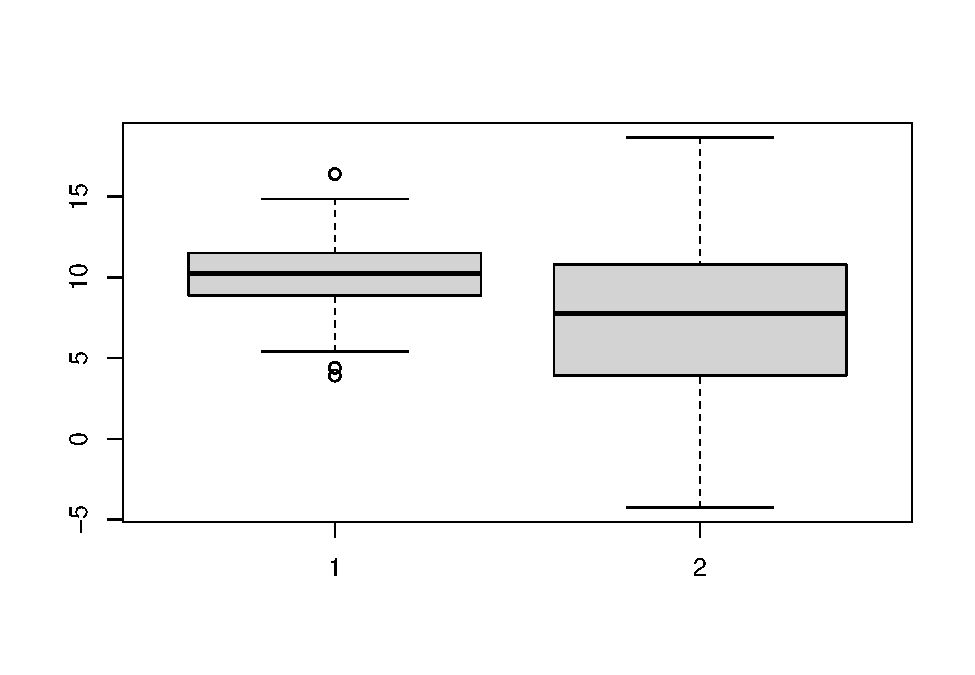
\includegraphics{taller_problemas_resueltos_extra_1_files/figure-latex/unnamed-chunk-8-1.pdf}

\begin{Shaded}
\begin{Highlighting}[]
\KeywordTok{library}\NormalTok{(car)}
\KeywordTok{par}\NormalTok{(}\DataTypeTok{mfrow=}\KeywordTok{c}\NormalTok{(}\DecValTok{1}\NormalTok{,}\DecValTok{2}\NormalTok{))}
\KeywordTok{qqPlot}\NormalTok{(x1)}
\end{Highlighting}
\end{Shaded}

\begin{verbatim}
## [1] 18 64
\end{verbatim}

\begin{Shaded}
\begin{Highlighting}[]
\KeywordTok{qqPlot}\NormalTok{(x2)}
\end{Highlighting}
\end{Shaded}

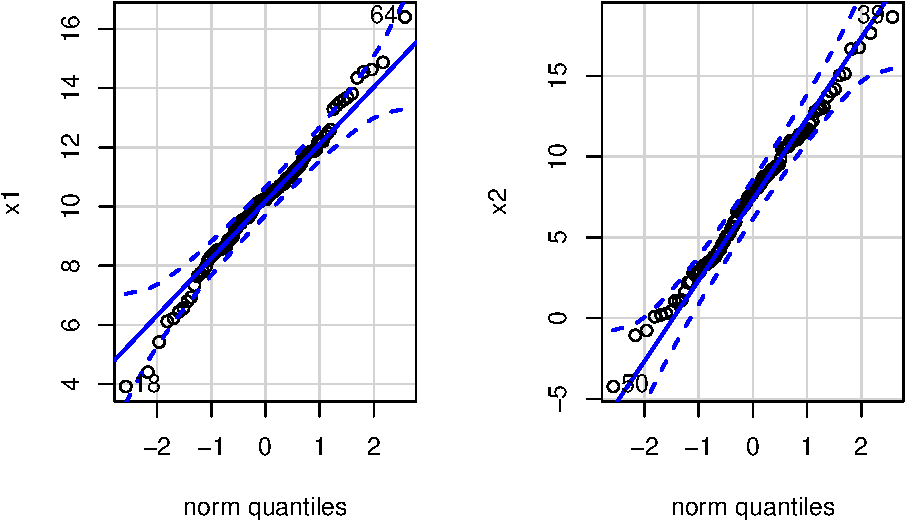
\includegraphics{taller_problemas_resueltos_extra_1_files/figure-latex/unnamed-chunk-8-2.pdf}

\begin{verbatim}
## [1] 50 39
\end{verbatim}

\begin{Shaded}
\begin{Highlighting}[]
\KeywordTok{par}\NormalTok{(}\DataTypeTok{mfrow=}\KeywordTok{c}\NormalTok{(}\DecValTok{1}\NormalTok{,}\DecValTok{1}\NormalTok{))}
\end{Highlighting}
\end{Shaded}

Realizamos algunos contrastes de hipótesis de igual de medias entre
ambas muestras

\begin{Shaded}
\begin{Highlighting}[]
\KeywordTok{t.test}\NormalTok{(x1,x2,}\DataTypeTok{var.equal =} \OtherTok{TRUE}\NormalTok{,}\DataTypeTok{alternative =} \StringTok{"greater"}\NormalTok{)}
\end{Highlighting}
\end{Shaded}

\begin{verbatim}
## 
##  Two Sample t-test
## 
## data:  x1 and x2
## t = 5.3009, df = 198, p-value = 0.0000001531
## alternative hypothesis: true difference in means is greater than 0
## 95 percent confidence interval:
##  1.844757      Inf
## sample estimates:
## mean of x mean of y 
## 10.217784  7.537402
\end{verbatim}

\begin{Shaded}
\begin{Highlighting}[]
\KeywordTok{t.test}\NormalTok{(x1,x2,}\DataTypeTok{var.equal =} \OtherTok{FALSE}\NormalTok{,}\DataTypeTok{alternative =} \StringTok{"two.sided"}\NormalTok{)}
\end{Highlighting}
\end{Shaded}

\begin{verbatim}
## 
##  Welch Two Sample t-test
## 
## data:  x1 and x2
## t = 5.3009, df = 144.56, p-value = 0.0000004221
## alternative hypothesis: true difference in means is not equal to 0
## 95 percent confidence interval:
##  1.680966 3.679797
## sample estimates:
## mean of x mean of y 
## 10.217784  7.537402
\end{verbatim}

\begin{Shaded}
\begin{Highlighting}[]
\KeywordTok{t.test}\NormalTok{(x1,x2,}\DataTypeTok{var.equal =} \OtherTok{TRUE}\NormalTok{)}
\end{Highlighting}
\end{Shaded}

\begin{verbatim}
## 
##  Two Sample t-test
## 
## data:  x1 and x2
## t = 5.3009, df = 198, p-value = 0.0000003061
## alternative hypothesis: true difference in means is not equal to 0
## 95 percent confidence interval:
##  1.683238 3.677526
## sample estimates:
## mean of x mean of y 
## 10.217784  7.537402
\end{verbatim}

Se pide

\begin{enumerate}
\def\labelenumi{\arabic{enumi}.}
\tightlist
\item
  ¿Cuál es la distribución y los parámetros de las muestras generadas?
\item
  ¿Qué muestran y cuál es la interpretación de los gráficos?
\item
  ¿Qué test contrasta si hay evidencia a favor de que las medias
  poblacionales de las notas en cada grupo sean distintas? Di qué código
  de los anteriores resuelve este test.
\item
  Para el test del apartado anterior dad las hipótesis nula y
  alternativa y redactar la conclusión del contraste.
\end{enumerate}

\hypertarget{soluciuxf3n-1}{%
\subsubsection{Solución}\label{soluciuxf3n-1}}

\textbf{Apartado 1}

Se generan dos muestras de poblaciones normales de medias 10 y 8 y
desviaciones típicas 2 y 4.

\textbf{Apartado 2} El primer gráficos es un diagrama de caja
(\emph{boxplot}) que compara las distribuciones de los datos. Vemos que
efectivamente la muestra 1 tiene una caja y unos bigotes más comprimidos
que la muestra 2 así que la primera tiene menos varianza. Vemos que los
valores medianos de la muestra 1 son más grandes que los de la muestra
2. Recordemos que la distribución normal es simétrica por lo que la
media y la mediana coinciden. La muestra 1 tiene valores atípicos en la
parte superior 1 y en la inferior parece que 2.

El segundo gráfico es un gráfico cuantil-cuantil o qqplot de normalidad.
Compara los cuantiles muestrales con los teóricos de una normal y nos da
un intervalo de confianza para esas observaciones.

Vemos que los cuantiles teóricos no difieren excesivamente de los
muestrales en cada una de las muestras y que muy pocos valores se
escapan de los intervalos de confianza esperados en el caso de
normalidad. Así que no hay motivo para pensar que las distribuciones de
ambas muestras proceden de poblaciones normales.

\textbf{Apartado 3}

El código es

\begin{verbatim}
t.test(x1,x2,var.equal = TRUE,alternative = "greater")
t.test(x1,x2,var.equal = FALSE,alternative = "two.sided")
t.test(x1,x2,var.equal = TRUE)
\end{verbatim}

El primer test contrasta para muestras independientes supuestas
varianzas desconocidas pero iguales \(H_0;\mu_1=\mu_2\) contra
\(H_1:\mu_1>\mu_2\). \textbf{Así que este TEST NO ES}

El segundo test contrasta para muestras independientes supuestas
varianzas desconocidas pero iguales \(H_0;\mu_1=\mu_2\) contra
\(H_1:\mu_1\not=\mu_2\). \textbf{Así que este TEST SÍ PUEDE SER}
contrasta contra medias distintas para el caso de varianzas distintas.

El tercer test contrasta para muestras independientes supuestas
varianzas desconocidas pero iguales \(H_0;\mu_1=\mu_2\) contra
\(H_1:\mu_1>\mu_2\) pues la opción por defecto de la función.
\textbf{Así que este TEST SÍ PUEDE SER} contra medias distintas para el
caso de varianzas iguales.

\textbf{Apartado 4} El contrastes es

\[\left\{\begin{array}{ll}H_0: & \mu_1=\mu_2\\ H_1: & \mu_1\not=\mu_2\end{array}\right.
\]

En los dos últimos test los \(p\)-valores son muy muy pequeños así que
hay evidencias en contra de la igualdad de medias entre las dos
muestras. Además claramente los intervalos de confianza no contienen al
cero.

\hypertarget{problema-3-bondad-de-ajuste.-la-ley-de-benford}{%
\subsection{Problema 3 : Bondad de ajuste. La ley de
Benford}\label{problema-3-bondad-de-ajuste.-la-ley-de-benford}}

La ley de Benford es una distribución discreta que siguen las
frecuencias de los primero dígitos significativos (de 1 a 9) de algunas
series de datos curiosas.

Sea una v.a. X con dominio \(D_X=\left\{1,2,3,4,5,6,7,8,9\right\}\)
diremos que sigue una ley de Benford si

\[P(X=x)=\log_{10} \left(1+\frac{1}{x}\right)\mbox{ para } x\in \left\{1,2,3,4,5,6,7,8,9\right\}.\]

Concretamente lo podemos hacer así

\begin{Shaded}
\begin{Highlighting}[]
\NormalTok{prob=}\KeywordTok{log10}\NormalTok{(}\DecValTok{1}\OperatorTok{+}\DecValTok{1}\OperatorTok{/}\KeywordTok{c}\NormalTok{(}\DecValTok{1}\OperatorTok{:}\DecValTok{9}\NormalTok{))}
\NormalTok{prob}
\end{Highlighting}
\end{Shaded}

\begin{verbatim}
## [1] 0.30103000 0.17609126 0.12493874 0.09691001 0.07918125 0.06694679 0.05799195
## [8] 0.05115252 0.04575749
\end{verbatim}

\begin{Shaded}
\begin{Highlighting}[]
\NormalTok{df=}\KeywordTok{data.frame}\NormalTok{(}\KeywordTok{rbind}\NormalTok{(prob))}
\CommentTok{\# Y hacemos una bonita tabla}
\KeywordTok{colnames}\NormalTok{(df)=}\KeywordTok{paste}\NormalTok{(}\StringTok{"Díg."}\NormalTok{,}\KeywordTok{c}\NormalTok{(}\DecValTok{1}\OperatorTok{:}\DecValTok{9}\NormalTok{),}\DataTypeTok{sep =}\StringTok{" "}\NormalTok{)}
\NormalTok{knitr}\OperatorTok{::}\KeywordTok{kable}\NormalTok{(df,}\DataTypeTok{format =}\StringTok{\textquotesingle{}markdown\textquotesingle{}}\NormalTok{)}
\end{Highlighting}
\end{Shaded}

\begin{longtable}[]{@{}lrrrrrrrrr@{}}
\toprule
\begin{minipage}[b]{0.04\columnwidth}\raggedright
\strut
\end{minipage} & \begin{minipage}[b]{0.06\columnwidth}\raggedleft
Díg. 1\strut
\end{minipage} & \begin{minipage}[b]{0.08\columnwidth}\raggedleft
Díg. 2\strut
\end{minipage} & \begin{minipage}[b]{0.08\columnwidth}\raggedleft
Díg. 3\strut
\end{minipage} & \begin{minipage}[b]{0.06\columnwidth}\raggedleft
Díg. 4\strut
\end{minipage} & \begin{minipage}[b]{0.08\columnwidth}\raggedleft
Díg. 5\strut
\end{minipage} & \begin{minipage}[b]{0.08\columnwidth}\raggedleft
Díg. 6\strut
\end{minipage} & \begin{minipage}[b]{0.08\columnwidth}\raggedleft
Díg. 7\strut
\end{minipage} & \begin{minipage}[b]{0.08\columnwidth}\raggedleft
Díg. 8\strut
\end{minipage} & \begin{minipage}[b]{0.08\columnwidth}\raggedleft
Díg. 9\strut
\end{minipage}\tabularnewline
\midrule
\endhead
\begin{minipage}[t]{0.04\columnwidth}\raggedright
prob\strut
\end{minipage} & \begin{minipage}[t]{0.06\columnwidth}\raggedleft
0.30103\strut
\end{minipage} & \begin{minipage}[t]{0.08\columnwidth}\raggedleft
0.1760913\strut
\end{minipage} & \begin{minipage}[t]{0.08\columnwidth}\raggedleft
0.1249387\strut
\end{minipage} & \begin{minipage}[t]{0.06\columnwidth}\raggedleft
0.09691\strut
\end{minipage} & \begin{minipage}[t]{0.08\columnwidth}\raggedleft
0.0791812\strut
\end{minipage} & \begin{minipage}[t]{0.08\columnwidth}\raggedleft
0.0669468\strut
\end{minipage} & \begin{minipage}[t]{0.08\columnwidth}\raggedleft
0.0579919\strut
\end{minipage} & \begin{minipage}[t]{0.08\columnwidth}\raggedleft
0.0511525\strut
\end{minipage} & \begin{minipage}[t]{0.08\columnwidth}\raggedleft
0.0457575\strut
\end{minipage}\tabularnewline
\bottomrule
\end{longtable}

En general esta distribución se suele encontrar en tablas de datos de
resultados de observaciones de funciones científicas, contabilidades,
cocientes de algunas distribuciones \ldots{}

Por ejemplo se dice que las potencias de números enteros siguen esa
distribución. Probemos con las potencias de 2. El siguiente código
calcula las potencias de 2 de 1 a 1000 y extrae los tres primeros
dígitos.

\begin{Shaded}
\begin{Highlighting}[]
\CommentTok{\# R puede según qué versión pasar los enteros  muy grande a reales. Para nuestros propósitos }
\CommentTok{\# es suficiente para extraer los tres primeros dígitos.}
\NormalTok{muestra\_pot\_}\DecValTok{2}\NormalTok{\_3digitos=}\KeywordTok{str\_sub}\NormalTok{(}\KeywordTok{as.character}\NormalTok{(}\DecValTok{2}\OperatorTok{\^{}}\KeywordTok{c}\NormalTok{(}\DecValTok{1}\OperatorTok{:}\DecValTok{1000}\NormalTok{)),}\DecValTok{1}\NormalTok{,}\DecValTok{3}\NormalTok{)}
\KeywordTok{head}\NormalTok{(muestra\_pot\_}\DecValTok{2}\NormalTok{\_3digitos)}
\end{Highlighting}
\end{Shaded}

\begin{verbatim}
## [1] "2"  "4"  "8"  "16" "32" "64"
\end{verbatim}

\begin{Shaded}
\begin{Highlighting}[]
\KeywordTok{tail}\NormalTok{(muestra\_pot\_}\DecValTok{2}\NormalTok{\_3digitos)}
\end{Highlighting}
\end{Shaded}

\begin{verbatim}
## [1] "334" "669" "133" "267" "535" "107"
\end{verbatim}

\begin{Shaded}
\begin{Highlighting}[]
\CommentTok{\#Construimos un data frame con tres columnas que nos dan el primer, }
\CommentTok{\#segundo y tercer dígito respectivamente.}
\NormalTok{df\_digitos=}\KeywordTok{data.frame}\NormalTok{(muestra\_pot\_}\DecValTok{2}\NormalTok{\_3digitos,}
                      \DataTypeTok{primer\_digito=}\KeywordTok{as.integer}\NormalTok{(}
                        \KeywordTok{substring}\NormalTok{(muestra\_pot\_}\DecValTok{2}\NormalTok{\_3digitos, }\DecValTok{1}\NormalTok{, }\DecValTok{1}\NormalTok{)),}
                      \DataTypeTok{segundo\_digito=}\KeywordTok{as.integer}\NormalTok{(}
                        \KeywordTok{substring}\NormalTok{(muestra\_pot\_}\DecValTok{2}\NormalTok{\_3digitos, }\DecValTok{2}\NormalTok{, }\DecValTok{2}\NormalTok{)),}
                      \DataTypeTok{tercer\_digito=}\KeywordTok{as.integer}\NormalTok{(}
                        \KeywordTok{substring}\NormalTok{(muestra\_pot\_}\DecValTok{2}\NormalTok{\_3digitos, }\DecValTok{3}\NormalTok{, }\DecValTok{3}\NormalTok{)))}
\KeywordTok{head}\NormalTok{(df\_digitos)}
\end{Highlighting}
\end{Shaded}

\begin{verbatim}
##   muestra_pot_2_3digitos primer_digito segundo_digito tercer_digito
## 1                      2             2             NA            NA
## 2                      4             4             NA            NA
## 3                      8             8             NA            NA
## 4                     16             1              6            NA
## 5                     32             3              2            NA
## 6                     64             6              4            NA
\end{verbatim}

Notad que los NA en el segundo y el tercer dígito corresponden a número
con uno o dos dígitos.

Se pide:

\begin{enumerate}
\def\labelenumi{\arabic{enumi}.}
\tightlist
\item
  Contrastad con un test \(\chi^2\) que el primer dígito sigue una ley
  de Benford. Notad que el primer dígito no puede ser 0. Resolved
  manualmente y con una función de \texttt{R}.\\
\item
  Contrastad con un test \(\chi^2\) que el segundo dígito sigue una ley
  de uniforme discreta. Notad que ahora si puede ser 0. Resolved con
  funciones de \texttt{R}.\\
\item
  Contrastad con un test \(\chi^2\) que el tercer dígito sigue una ley
  de uniforme discreta. Notad que ahora si puede ser 0. Resolved con
  manualmente calculado las frecuencias esperadas y observadas, el
  estadístico de contraste y el \(p\)-valor utilizando \texttt{R}.
  Comprobad que vuestros resultados coinciden con los de la función de
  \texttt{R} que calcula este contraste.\\
\item
  Dibujad con \texttt{R} para los apartados 1 y 2 los diagramas de
  frecuencias esperados y observados. Comentad estos gráficos
\end{enumerate}

\hypertarget{soluciuxf3n-2}{%
\subsubsection{Solución}\label{soluciuxf3n-2}}

\textbf{Apartado 1} El contraste que nos piden es \[
\left\{
\begin{array}{ll}
H_0: &  \mbox{ El primer dígito de las 1000 primeras potencias de 2 sigue una ley Benford,}\\
H_1: & \mbox{sigue cualquier otra distribución}.
\end{array}
\right.
\]

El siguiente código resuelve el tes de forma manual calculando el
estadístico y el \(p\)-valor

\begin{Shaded}
\begin{Highlighting}[]
\NormalTok{prob=}\KeywordTok{log10}\NormalTok{(}\DecValTok{1}\OperatorTok{+}\DecValTok{1}\OperatorTok{/}\NormalTok{(}\DecValTok{1}\OperatorTok{:}\DecValTok{9}\NormalTok{))}
\NormalTok{prob\_benford=prob}
\NormalTok{n=}\DecValTok{1000}
\NormalTok{frec\_esp\_benford=n}\OperatorTok{*}\NormalTok{prob\_benford}
\NormalTok{frec\_esp\_benford}
\end{Highlighting}
\end{Shaded}

\begin{verbatim}
## [1] 301.03000 176.09126 124.93874  96.91001  79.18125  66.94679  57.99195
## [8]  51.15252  45.75749
\end{verbatim}

\begin{Shaded}
\begin{Highlighting}[]
\NormalTok{frec\_obs\_primer=}\KeywordTok{table}\NormalTok{(df\_digitos}\OperatorTok{$}\NormalTok{primer\_digito)}
\NormalTok{frec\_obs\_primer}
\end{Highlighting}
\end{Shaded}

\begin{verbatim}
## 
##   1   2   3   4   5   6   7   8   9 
## 301 176 125  97  79  69  56  52  45
\end{verbatim}

\begin{Shaded}
\begin{Highlighting}[]
\NormalTok{chi2\_est=}\KeywordTok{sum}\NormalTok{((frec\_obs\_primer}\OperatorTok{{-}}\NormalTok{frec\_esp\_benford)}\OperatorTok{\^{}}\DecValTok{2}\OperatorTok{/}\NormalTok{frec\_esp\_benford)}
\NormalTok{chi2\_est}
\end{Highlighting}
\end{Shaded}

\begin{verbatim}
## [1] 0.1585506
\end{verbatim}

\begin{Shaded}
\begin{Highlighting}[]
\KeywordTok{pchisq}\NormalTok{(chi2\_est,}\DecValTok{9{-}1}\NormalTok{,}\DataTypeTok{lower.tail =} \OtherTok{FALSE}\NormalTok{)}
\end{Highlighting}
\end{Shaded}

\begin{verbatim}
## [1] 0.9999985
\end{verbatim}

La función de R que resuelve el test es

\begin{Shaded}
\begin{Highlighting}[]
\KeywordTok{chisq.test}\NormalTok{(frec\_obs\_primer,}\DataTypeTok{p=}\NormalTok{prob\_benford)}
\end{Highlighting}
\end{Shaded}

\begin{verbatim}
## 
##  Chi-squared test for given probabilities
## 
## data:  frec_obs_primer
## X-squared = 0.15855, df = 8, p-value = 1
\end{verbatim}

Obtenemos los mismos resultados. El \(p\) valor es muy alto. No podemos
rechazar que el primer dígito de las 1000 primeras potencias enteras de
2 siga una ley de distribución de Benford.

\textbf{Apartado 2}

El contraste que nos piden es \[
\left\{
\begin{array}{ll}
H_0: &  \mbox{ El segundo dígito de las 1000 primeras potencias de 2 sigue una ley uniforme,}\\
H_1: & \mbox{sigue cualquier otra distribución}.
\end{array}
\right.
\]

Procedemos de forma similar al caso anterior. De forma manual el cálculo
es

\begin{Shaded}
\begin{Highlighting}[]
\NormalTok{prob\_unif=}\KeywordTok{rep}\NormalTok{(}\DecValTok{1}\OperatorTok{/}\DecValTok{10}\NormalTok{,}\DecValTok{10}\NormalTok{)}
\NormalTok{prob\_unif}
\end{Highlighting}
\end{Shaded}

\begin{verbatim}
##  [1] 0.1 0.1 0.1 0.1 0.1 0.1 0.1 0.1 0.1 0.1
\end{verbatim}

\begin{Shaded}
\begin{Highlighting}[]
\NormalTok{segundo\_digito=}\KeywordTok{na.omit}\NormalTok{(df\_digitos}\OperatorTok{$}\NormalTok{segundo\_digito)}
\NormalTok{n=}\KeywordTok{length}\NormalTok{(segundo\_digito) }
\NormalTok{n}
\end{Highlighting}
\end{Shaded}

\begin{verbatim}
## [1] 997
\end{verbatim}

\begin{Shaded}
\begin{Highlighting}[]
\NormalTok{frec\_esp\_uniforme=n}\OperatorTok{*}\NormalTok{prob\_unif}
\NormalTok{frec\_esp\_uniforme }
\end{Highlighting}
\end{Shaded}

\begin{verbatim}
##  [1] 99.7 99.7 99.7 99.7 99.7 99.7 99.7 99.7 99.7 99.7
\end{verbatim}

\begin{Shaded}
\begin{Highlighting}[]
\NormalTok{frec\_obs\_segundo=}\KeywordTok{table}\NormalTok{(segundo\_digito)}
\NormalTok{frec\_obs\_segundo}
\end{Highlighting}
\end{Shaded}

\begin{verbatim}
## segundo_digito
##   0   1   2   3   4   5   6   7   8   9 
## 121 112 109 108  98  95  94  91  83  86
\end{verbatim}

\begin{Shaded}
\begin{Highlighting}[]
\NormalTok{chi2\_est=}\KeywordTok{sum}\NormalTok{((frec\_obs\_segundo}\OperatorTok{{-}}\NormalTok{frec\_esp\_uniforme)}\OperatorTok{\^{}}\DecValTok{2}\OperatorTok{/}\NormalTok{frec\_esp\_uniforme)}
\NormalTok{chi2\_est}
\end{Highlighting}
\end{Shaded}

\begin{verbatim}
## [1] 13.64193
\end{verbatim}

\begin{Shaded}
\begin{Highlighting}[]
\DecValTok{1}\OperatorTok{{-}}\KeywordTok{pchisq}\NormalTok{(chi2\_est,}\DecValTok{10{-}1}\NormalTok{)}
\end{Highlighting}
\end{Shaded}

\begin{verbatim}
## [1] 0.1356449
\end{verbatim}

\begin{Shaded}
\begin{Highlighting}[]
\KeywordTok{pchisq}\NormalTok{(chi2\_est,}\DecValTok{10{-}1}\NormalTok{,}\DataTypeTok{lower.tail =} \OtherTok{FALSE}\NormalTok{)}
\end{Highlighting}
\end{Shaded}

\begin{verbatim}
## [1] 0.1356449
\end{verbatim}

Con la función \texttt{chisq.test} obtenemos los mismo resultados

\begin{Shaded}
\begin{Highlighting}[]
\KeywordTok{chisq.test}\NormalTok{(frec\_obs\_segundo,}\DataTypeTok{p=}\NormalTok{prob\_unif)}
\end{Highlighting}
\end{Shaded}

\begin{verbatim}
## 
##  Chi-squared test for given probabilities
## 
## data:  frec_obs_segundo
## X-squared = 13.642, df = 9, p-value = 0.1356
\end{verbatim}

Para el segundo dígito con un \(p\)-valor de \(0.1356\) no podemos
rechazar que el segundo dígito siga una ley uniforme.

\textbf{Apartado 3}

El contraste que nos piden es \[
\left\{
\begin{array}{ll}
H_0: &  \mbox{ El tercer dígito de las 1000 primeras potencias de 2 sigue una ley uniforme,}\\
H_1: & \mbox{sigue cualquier otra distribución}.
\end{array}
\right.
\]

Procedemos de forma similar al caso anterior. De forma manual el cálculo
es

\begin{Shaded}
\begin{Highlighting}[]
\NormalTok{prob\_unif=}\KeywordTok{rep}\NormalTok{(}\DecValTok{1}\OperatorTok{/}\DecValTok{10}\NormalTok{,}\DecValTok{10}\NormalTok{)}
\NormalTok{prob\_unif}
\end{Highlighting}
\end{Shaded}

\begin{verbatim}
##  [1] 0.1 0.1 0.1 0.1 0.1 0.1 0.1 0.1 0.1 0.1
\end{verbatim}

\begin{Shaded}
\begin{Highlighting}[]
\NormalTok{tercer\_digito=}\KeywordTok{na.omit}\NormalTok{(df\_digitos}\OperatorTok{$}\NormalTok{tercer\_digito)}
\NormalTok{n=}\KeywordTok{length}\NormalTok{(tercer\_digito) }
\NormalTok{n}
\end{Highlighting}
\end{Shaded}

\begin{verbatim}
## [1] 994
\end{verbatim}

\begin{Shaded}
\begin{Highlighting}[]
\NormalTok{frec\_esp\_uniforme=n}\OperatorTok{*}\NormalTok{prob\_unif}
\NormalTok{frec\_esp\_uniforme }
\end{Highlighting}
\end{Shaded}

\begin{verbatim}
##  [1] 99.4 99.4 99.4 99.4 99.4 99.4 99.4 99.4 99.4 99.4
\end{verbatim}

\begin{Shaded}
\begin{Highlighting}[]
\NormalTok{frec\_obs\_tercer=}\KeywordTok{table}\NormalTok{(tercer\_digito)}
\NormalTok{frec\_obs\_tercer}
\end{Highlighting}
\end{Shaded}

\begin{verbatim}
## tercer_digito
##   0   1   2   3   4   5   6   7   8   9 
##  96 101  88 116  97  90 110  92  95 109
\end{verbatim}

\begin{Shaded}
\begin{Highlighting}[]
\NormalTok{chi2\_est=}\KeywordTok{sum}\NormalTok{((frec\_obs\_tercer}\OperatorTok{{-}}\NormalTok{frec\_esp\_uniforme)}\OperatorTok{\^{}}\DecValTok{2}\OperatorTok{/}\NormalTok{frec\_esp\_uniforme)}
\NormalTok{chi2\_est}
\end{Highlighting}
\end{Shaded}

\begin{verbatim}
## [1] 7.971831
\end{verbatim}

\begin{Shaded}
\begin{Highlighting}[]
\DecValTok{1}\OperatorTok{{-}}\KeywordTok{pchisq}\NormalTok{(chi2\_est,}\DecValTok{10{-}1}\NormalTok{)}
\end{Highlighting}
\end{Shaded}

\begin{verbatim}
## [1] 0.5369875
\end{verbatim}

\begin{Shaded}
\begin{Highlighting}[]
\KeywordTok{pchisq}\NormalTok{(chi2\_est,}\DecValTok{10{-}1}\NormalTok{,}\DataTypeTok{lower.tail =} \OtherTok{FALSE}\NormalTok{)}
\end{Highlighting}
\end{Shaded}

\begin{verbatim}
## [1] 0.5369875
\end{verbatim}

Con la función \texttt{chisq.test} obtenemos los mismo resultados

\begin{Shaded}
\begin{Highlighting}[]
\KeywordTok{chisq.test}\NormalTok{(frec\_obs\_tercer,}\DataTypeTok{p=}\NormalTok{prob\_unif)}
\end{Highlighting}
\end{Shaded}

\begin{verbatim}
## 
##  Chi-squared test for given probabilities
## 
## data:  frec_obs_tercer
## X-squared = 7.9718, df = 9, p-value = 0.537
\end{verbatim}

Para el segundo dígito con un \(p\)-valor alto \(0.537\) no podemos
rechazar que el tercer dígito siga una ley uniforme.

\textbf{Apartado 4}

Una gráfica comparando las frecuencias

\begin{Shaded}
\begin{Highlighting}[]
\KeywordTok{barplot}\NormalTok{(}\KeywordTok{rbind}\NormalTok{(frec\_esp\_benford,frec\_obs\_primer),}
        \DataTypeTok{beside=}\OtherTok{TRUE}\NormalTok{,}\DataTypeTok{col=}\KeywordTok{c}\NormalTok{(}\StringTok{"red"}\NormalTok{,}\StringTok{"blue"}\NormalTok{),}
        \DataTypeTok{main=}\StringTok{"Frecuencias observadas y}\CharTok{\textbackslash{}n}\StringTok{ esperadas del primer dígito"}\NormalTok{,}
        \DataTypeTok{cex.names =}\FloatTok{0.6}\NormalTok{,}\DataTypeTok{xlab=}\StringTok{"Dígito"}\NormalTok{,}\DataTypeTok{ylab=}\StringTok{"Frecuencia absoluta"}\NormalTok{)}
\KeywordTok{legend}\NormalTok{(}\StringTok{"topright"}\NormalTok{,}\DataTypeTok{legen=}\KeywordTok{c}\NormalTok{(}\StringTok{"Frecuencias  observadas"}\NormalTok{,}
                          \StringTok{"Frecuencias esperadas ley de Benfor"}\NormalTok{),}\DataTypeTok{pch=}\DecValTok{19}\NormalTok{,}\DataTypeTok{col=}\KeywordTok{c}\NormalTok{(}\StringTok{"red"}\NormalTok{,}\StringTok{"blue"}\NormalTok{),}
       \DataTypeTok{cex=}\FloatTok{0.8}\NormalTok{)}
\end{Highlighting}
\end{Shaded}

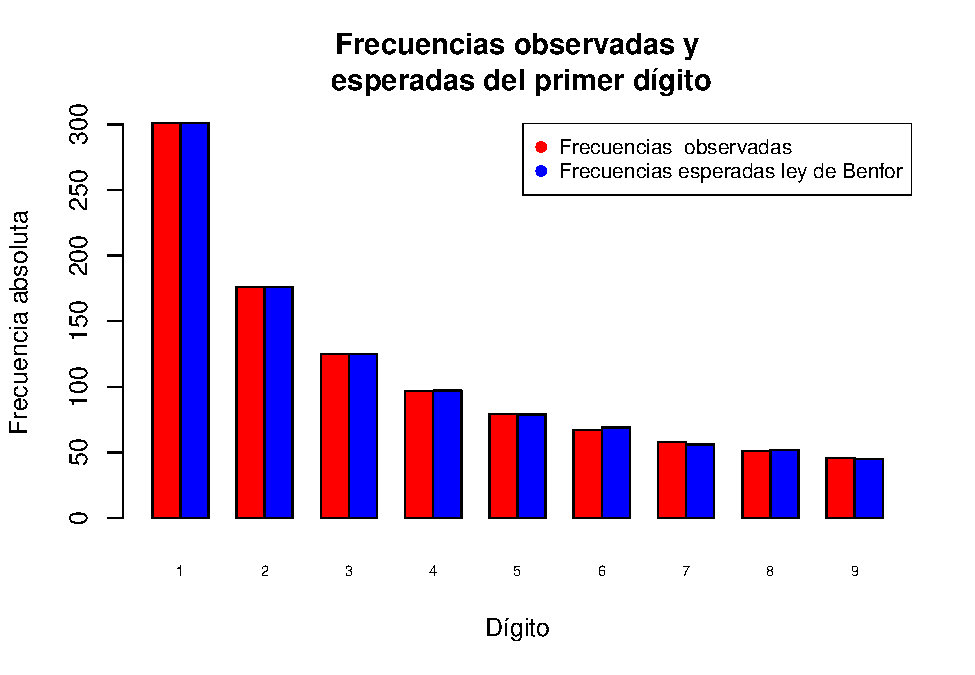
\includegraphics{taller_problemas_resueltos_extra_1_files/figure-latex/unnamed-chunk-15-1.pdf}

\begin{Shaded}
\begin{Highlighting}[]
\KeywordTok{barplot}\NormalTok{(}\KeywordTok{rbind}\NormalTok{(frec\_esp\_uniforme,frec\_obs\_segundo),}
        \DataTypeTok{beside=}\OtherTok{TRUE}\NormalTok{,}\DataTypeTok{col=}\KeywordTok{c}\NormalTok{(}\StringTok{"red"}\NormalTok{,}\StringTok{"blue"}\NormalTok{),}
        \DataTypeTok{main=}\StringTok{"Frecuencias observadas y}\CharTok{\textbackslash{}n}\StringTok{ esperadas del segundo dígito"}\NormalTok{,}
        \DataTypeTok{cex.names =}\FloatTok{0.6}\NormalTok{,}\DataTypeTok{xlab=}\StringTok{"Dígito"}\NormalTok{,}\DataTypeTok{ylab=}\StringTok{"Frecuencia absoluta"}\NormalTok{)}
\KeywordTok{legend}\NormalTok{(}\StringTok{"topright"}\NormalTok{,}\DataTypeTok{legen=}\KeywordTok{c}\NormalTok{(}\StringTok{"Frecuencias  observadas"}\NormalTok{,}
                          \StringTok{"Frecuencias esperadas uniformes"}\NormalTok{),}\DataTypeTok{pch=}\DecValTok{19}\NormalTok{,}\DataTypeTok{col=}\KeywordTok{c}\NormalTok{(}\StringTok{"red"}\NormalTok{,}\StringTok{"blue"}\NormalTok{),}
       \DataTypeTok{cex=}\FloatTok{0.6}\NormalTok{)}
\end{Highlighting}
\end{Shaded}

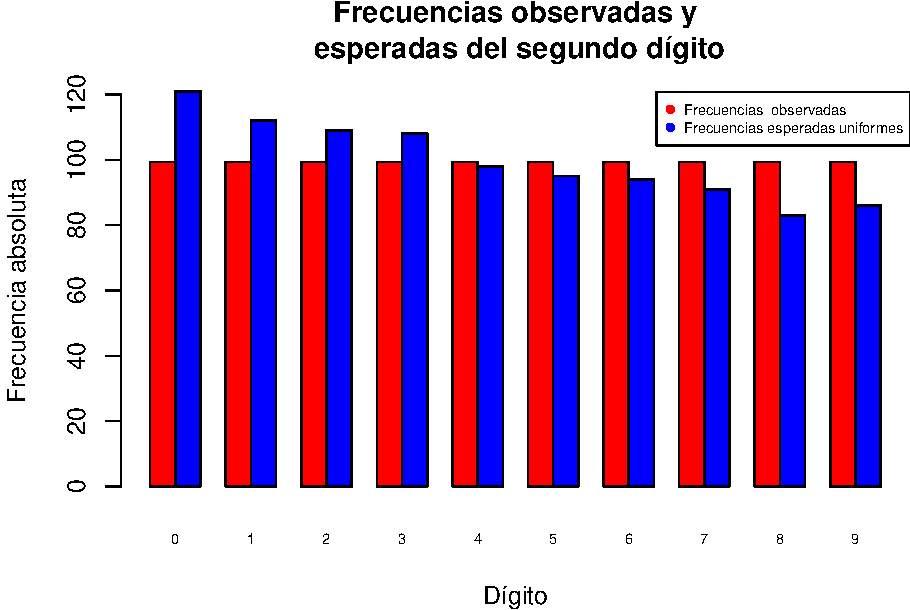
\includegraphics{taller_problemas_resueltos_extra_1_files/figure-latex/unnamed-chunk-15-2.pdf}

\hypertarget{problema-4-homegeneidad-e-independencia}{%
\subsection{Problema 4 : Homegeneidad e
independencia}\label{problema-4-homegeneidad-e-independencia}}

Queremos analiza los resultados de aprendizaje con tres tecnologías.
Para ello se seleccionan 3 muestras de 50 estudiantes y se les somete a
evaluación después de un curso.

\begin{Shaded}
\begin{Highlighting}[]
\KeywordTok{set.seed}\NormalTok{(}\DecValTok{2020}\NormalTok{)}
\NormalTok{nota=}\KeywordTok{factor}\NormalTok{(}\KeywordTok{sample}\NormalTok{(}\KeywordTok{c}\NormalTok{(}\DecValTok{1}\NormalTok{,}\DecValTok{2}\NormalTok{,}\DecValTok{3}\NormalTok{,}\DecValTok{4}\NormalTok{),}\DataTypeTok{p=}\KeywordTok{c}\NormalTok{(}\FloatTok{0.1}\NormalTok{,}\FloatTok{0.4}\NormalTok{,}\FloatTok{0.3}\NormalTok{,}\FloatTok{0.2}\NormalTok{),}\DataTypeTok{replace=}\OtherTok{TRUE}\NormalTok{,}\DataTypeTok{size=}\DecValTok{150}\NormalTok{),}
            \DataTypeTok{labels=}\KeywordTok{c}\NormalTok{(}\StringTok{"S"}\NormalTok{,}\StringTok{"A"}\NormalTok{,}\StringTok{"N"}\NormalTok{,}\StringTok{"E"}\NormalTok{))}
\NormalTok{tecnologia=}\KeywordTok{rep}\NormalTok{(}\KeywordTok{c}\NormalTok{(}\StringTok{"Mathematica"}\NormalTok{,}\StringTok{"R"}\NormalTok{,}\StringTok{"Python"}\NormalTok{),}\DataTypeTok{each=}\DecValTok{50}\NormalTok{)}
\NormalTok{frec=}\KeywordTok{table}\NormalTok{(nota,tecnologia)}
\NormalTok{frec}
\end{Highlighting}
\end{Shaded}

\begin{verbatim}
##     tecnologia
## nota Mathematica Python  R
##    S           7      6  2
##    A          18     15 22
##    N          15     20 18
##    E          10      9  8
\end{verbatim}

\begin{Shaded}
\begin{Highlighting}[]
\NormalTok{col\_frec=}\KeywordTok{colSums}\NormalTok{(frec)}
\NormalTok{col\_frec}
\end{Highlighting}
\end{Shaded}

\begin{verbatim}
## Mathematica      Python           R 
##          50          50          50
\end{verbatim}

\begin{Shaded}
\begin{Highlighting}[]
\NormalTok{row\_frec=}\KeywordTok{rowSums}\NormalTok{(frec)}
\NormalTok{row\_frec}
\end{Highlighting}
\end{Shaded}

\begin{verbatim}
##  S  A  N  E 
## 15 55 53 27
\end{verbatim}

\begin{Shaded}
\begin{Highlighting}[]
\NormalTok{N=}\KeywordTok{sum}\NormalTok{(frec)}
\NormalTok{teoricas=row\_frec}\OperatorTok{\%*\%}\KeywordTok{t}\NormalTok{(col\_frec)}\OperatorTok{/}\NormalTok{N}
\NormalTok{teoricas}
\end{Highlighting}
\end{Shaded}

\begin{verbatim}
##      Mathematica   Python        R
## [1,]     5.00000  5.00000  5.00000
## [2,]    18.33333 18.33333 18.33333
## [3,]    17.66667 17.66667 17.66667
## [4,]     9.00000  9.00000  9.00000
\end{verbatim}

\begin{Shaded}
\begin{Highlighting}[]
\KeywordTok{dim}\NormalTok{(frec)}
\end{Highlighting}
\end{Shaded}

\begin{verbatim}
## [1] 4 3
\end{verbatim}

\begin{Shaded}
\begin{Highlighting}[]
\KeywordTok{dim}\NormalTok{(teoricas)}
\end{Highlighting}
\end{Shaded}

\begin{verbatim}
## [1] 4 3
\end{verbatim}

\begin{Shaded}
\begin{Highlighting}[]
\KeywordTok{sum}\NormalTok{((frec}\OperatorTok{{-}}\NormalTok{teoricas)}\OperatorTok{\^{}}\DecValTok{2}\OperatorTok{/}\NormalTok{teoricas)}
\end{Highlighting}
\end{Shaded}

\begin{verbatim}
## [1] 5.084658
\end{verbatim}

\begin{Shaded}
\begin{Highlighting}[]
\KeywordTok{chisq.test}\NormalTok{(}\KeywordTok{table}\NormalTok{(nota,tecnologia))}
\end{Highlighting}
\end{Shaded}

\begin{verbatim}
## 
##  Pearson's Chi-squared test
## 
## data:  table(nota, tecnologia)
## X-squared = 5.0847, df = 6, p-value = 0.533
\end{verbatim}

Se pide

\begin{enumerate}
\def\labelenumi{\arabic{enumi}.}
\tightlist
\item
  Discutid si hacemos un contraste de independencia o de homogeneidad de
  las distribuciones de las notas por tecnología. Escribid las hipótesis
  del contraste.
\item
  Interpretad la función \texttt{chisq.test} y resolved el contraste.
\item
  Interpretad \texttt{teoricas=row\_frec\%*\%t(col\_frec)/N} reproducid
  manualmente el segundo resultado de la primera fila.
\end{enumerate}

\hypertarget{soluciuxf3n-3}{%
\subsubsection{Solución}\label{soluciuxf3n-3}}

\textbf{Apartado 1}

Podemos plantear dos hipótesis distintas. La primera es que la
calificación obtenidas es independiente de la tecnología, la segunda es
las distribuciones en las 4 clases de notas son las mismas para cada
tecnología. En el primer caso es un contraste de independencia y en el
segundo es de homogeneidad.

Podemos optar en este caso por cualquiera de los dos. Yo he optado por
el de independencia

así que la hipótesis \(H_0\): la nota obtenida es independientes ce la
tecnología del curso, contra que no lo es.

\textbf{Apartado 2} Para el contraste de independencia (o el de
homogeneidad) hay que pasar una tabla de contingencia a la función
\texttt{chisq.test} eso es lo que hacemos

\begin{Shaded}
\begin{Highlighting}[]
\KeywordTok{table}\NormalTok{(nota,tecnologia)}
\end{Highlighting}
\end{Shaded}

\begin{verbatim}
##     tecnologia
## nota Mathematica Python  R
##    S           7      6  2
##    A          18     15 22
##    N          15     20 18
##    E          10      9  8
\end{verbatim}

\begin{Shaded}
\begin{Highlighting}[]
\KeywordTok{chisq.test}\NormalTok{(}\KeywordTok{table}\NormalTok{(nota,tecnologia))}
\end{Highlighting}
\end{Shaded}

\begin{verbatim}
## 
##  Pearson's Chi-squared test
## 
## data:  table(nota, tecnologia)
## X-squared = 5.0847, df = 6, p-value = 0.533
\end{verbatim}

El \(p\)-valor obtenido es grande así que no podemos rechazar la
hipótesis nula las calificaciones obtenidas no dependen del programa
utilizado en el curso.

\textbf{Apartado 3}

La expresión \texttt{teoricas=row\_frec\%*\%t(col\_frec)/N}

\begin{Shaded}
\begin{Highlighting}[]
\NormalTok{row\_frec  }
\end{Highlighting}
\end{Shaded}

\begin{verbatim}
##  S  A  N  E 
## 15 55 53 27
\end{verbatim}

\begin{Shaded}
\begin{Highlighting}[]
\NormalTok{col\_frec}
\end{Highlighting}
\end{Shaded}

\begin{verbatim}
## Mathematica      Python           R 
##          50          50          50
\end{verbatim}

\begin{Shaded}
\begin{Highlighting}[]
\NormalTok{row\_frec}\OperatorTok{\%*\%}\KeywordTok{t}\NormalTok{(col\_frec)}
\end{Highlighting}
\end{Shaded}

\begin{verbatim}
##      Mathematica Python    R
## [1,]         750    750  750
## [2,]        2750   2750 2750
## [3,]        2650   2650 2650
## [4,]        1350   1350 1350
\end{verbatim}

\begin{Shaded}
\begin{Highlighting}[]
\NormalTok{row\_frec}\OperatorTok{\%*\%}\KeywordTok{t}\NormalTok{(col\_frec)}\OperatorTok{/}\NormalTok{N}
\end{Highlighting}
\end{Shaded}

\begin{verbatim}
##      Mathematica   Python        R
## [1,]     5.00000  5.00000  5.00000
## [2,]    18.33333 18.33333 18.33333
## [3,]    17.66667 17.66667 17.66667
## [4,]     9.00000  9.00000  9.00000
\end{verbatim}

Así que \texttt{row\_frec\%*\%t(col\_frec)} calcula el producto de las
frecuencia marginal por filas y columnas.

Por ejemplo la segunda fila es \(2750= 50\cdot 55\) en los tres casos

Por último al dividir por \(N=150\) el tamaño total de las muestra
obtenemos las frecuencias esperadas en el caso de independencia
\(2750/150=18.33333\).

\hypertarget{problema-5-anova-notas-numuxe9ricas-de-tres-grupos.}{%
\subsection{Problema 5 : ANOVA notas numéricas de tres
grupos.}\label{problema-5-anova-notas-numuxe9ricas-de-tres-grupos.}}

El siguiente código nos da las notas numéricas (variable \texttt{nota})
de los mismos ejercicios para tres tecnologías en tres muestra
independientes de estudiantes de estas tres tecnologías diferentes

\begin{Shaded}
\begin{Highlighting}[]
\KeywordTok{head}\NormalTok{(nota)}
\end{Highlighting}
\end{Shaded}

\begin{verbatim}
## [1] 79.424303 77.538709 42.549421 41.739852  0.086642 88.014337
\end{verbatim}

\begin{Shaded}
\begin{Highlighting}[]
\KeywordTok{library}\NormalTok{(nortest)}
\KeywordTok{lillie.test}\NormalTok{(nota[tecnologia}\OperatorTok{==}\StringTok{"Mathematica"}\NormalTok{])}
\end{Highlighting}
\end{Shaded}

\begin{verbatim}
## 
##  Lilliefors (Kolmogorov-Smirnov) normality test
## 
## data:  nota[tecnologia == "Mathematica"]
## D = 0.08739, p-value = 0.4436
\end{verbatim}

\begin{Shaded}
\begin{Highlighting}[]
\KeywordTok{lillie.test}\NormalTok{(nota[tecnologia}\OperatorTok{==}\StringTok{"R"}\NormalTok{])}
\end{Highlighting}
\end{Shaded}

\begin{verbatim}
## 
##  Lilliefors (Kolmogorov-Smirnov) normality test
## 
## data:  nota[tecnologia == "R"]
## D = 0.082139, p-value = 0.5449
\end{verbatim}

\begin{Shaded}
\begin{Highlighting}[]
\KeywordTok{lillie.test}\NormalTok{(nota[tecnologia}\OperatorTok{==}\StringTok{"Python"}\NormalTok{])}
\end{Highlighting}
\end{Shaded}

\begin{verbatim}
## 
##  Lilliefors (Kolmogorov-Smirnov) normality test
## 
## data:  nota[tecnologia == "Python"]
## D = 0.089681, p-value = 0.4019
\end{verbatim}

\begin{Shaded}
\begin{Highlighting}[]
\KeywordTok{lillie.test}\NormalTok{(nota)}
\end{Highlighting}
\end{Shaded}

\begin{verbatim}
## 
##  Lilliefors (Kolmogorov-Smirnov) normality test
## 
## data:  nota
## D = 0.056381, p-value = 0.2885
\end{verbatim}

\begin{Shaded}
\begin{Highlighting}[]
\KeywordTok{bartlett.test}\NormalTok{(nota}\OperatorTok{\textasciitilde{}}\NormalTok{tecnologia)}
\end{Highlighting}
\end{Shaded}

\begin{verbatim}
## 
##  Bartlett test of homogeneity of variances
## 
## data:  nota by tecnologia
## Bartlett's K-squared = 0.50309, df = 2, p-value = 0.7776
\end{verbatim}

\begin{Shaded}
\begin{Highlighting}[]
\KeywordTok{library}\NormalTok{(car)}
\KeywordTok{leveneTest}\NormalTok{(nota}\OperatorTok{\textasciitilde{}}\KeywordTok{as.factor}\NormalTok{(tecnologia))}
\end{Highlighting}
\end{Shaded}

\begin{verbatim}
## Levene's Test for Homogeneity of Variance (center = median)
##        Df F value Pr(>F)
## group   2  0.3881  0.679
##       147
\end{verbatim}

\begin{Shaded}
\begin{Highlighting}[]
\NormalTok{sol\_aov=}\KeywordTok{aov}\NormalTok{(nota}\OperatorTok{\textasciitilde{}}\KeywordTok{as.factor}\NormalTok{(tecnologia))}
\NormalTok{sol\_aov}
\end{Highlighting}
\end{Shaded}

\begin{verbatim}
## Call:
##    aov(formula = nota ~ as.factor(tecnologia))
## 
## Terms:
##                 as.factor(tecnologia) Residuals
## Sum of Squares                 837.39 123445.06
## Deg. of Freedom                     2       147
## 
## Residual standard error: 28.97865
## Estimated effects may be unbalanced
\end{verbatim}

Del \texttt{summary(sol\_aov)} os damos la salida a falta de algunos de
los valores

\begin{verbatim}
> summary(sol_aov)
                      Df Sum Sq Mean Sq F value Pr(>F)
as.factor(tecnologia) ---    837   418.7   ---  ---
Residuals             --- 123445   839.8                          
\end{verbatim}

\begin{Shaded}
\begin{Highlighting}[]
\KeywordTok{pairwise.t.test}\NormalTok{(nota,}\KeywordTok{as.factor}\NormalTok{(tecnologia),}\DataTypeTok{p.adjust.method =} \StringTok{"none"}\NormalTok{)}
\end{Highlighting}
\end{Shaded}

\begin{verbatim}
## 
##  Pairwise comparisons using t tests with pooled SD 
## 
## data:  nota and as.factor(tecnologia) 
## 
##        Mathematica Python
## Python 0.35        -     
## R      0.89        0.43  
## 
## P value adjustment method: none
\end{verbatim}

\begin{Shaded}
\begin{Highlighting}[]
\KeywordTok{pairwise.t.test}\NormalTok{(nota,}\KeywordTok{as.factor}\NormalTok{(tecnologia),}\DataTypeTok{p.adjust.method =} \StringTok{"bonferroni"}\NormalTok{)}
\end{Highlighting}
\end{Shaded}

\begin{verbatim}
## 
##  Pairwise comparisons using t tests with pooled SD 
## 
## data:  nota and as.factor(tecnologia) 
## 
##        Mathematica Python
## Python 1           -     
## R      1           1     
## 
## P value adjustment method: bonferroni
\end{verbatim}

Se pide

\begin{enumerate}
\def\labelenumi{\arabic{enumi}.}
\tightlist
\item
  ¿Podemos asegurar que la muestras son normales en cada grupo? ¿y son
  homocedásticas? Sea cual sea la respuesta justificad que parte del
  código la confirma.
\item
  La función \texttt{aov} que test calcula. Escribid formalmente la
  hipótesis nula y la alternativa.
\item
  Calcula la tabla de ANOVA y resuelve el test.
\item
  ¿Qué contrates realiza la función \texttt{pairwise.t.test}? Utilizando
  los resultados anteriores aplicad e interpretad los contrates del
  apartado anterior utilizando el ajuste de Holm.
\end{enumerate}

\hypertarget{soluciuxf3n-4}{%
\subsubsection{Solución}\label{soluciuxf3n-4}}

\textbf{Apartado 1} Este código es el que pasa un test de normalidad con
la función \texttt{lillie.test} para la distribución de notas en cada
una de las tecnologías

\begin{Shaded}
\begin{Highlighting}[]
\KeywordTok{head}\NormalTok{(nota)}
\end{Highlighting}
\end{Shaded}

\begin{verbatim}
## [1] 79.424303 77.538709 42.549421 41.739852  0.086642 88.014337
\end{verbatim}

\begin{Shaded}
\begin{Highlighting}[]
\KeywordTok{library}\NormalTok{(nortest)}
\KeywordTok{lillie.test}\NormalTok{(nota[tecnologia}\OperatorTok{==}\StringTok{"Mathematica"}\NormalTok{])}
\end{Highlighting}
\end{Shaded}

\begin{verbatim}
## 
##  Lilliefors (Kolmogorov-Smirnov) normality test
## 
## data:  nota[tecnologia == "Mathematica"]
## D = 0.08739, p-value = 0.4436
\end{verbatim}

\begin{Shaded}
\begin{Highlighting}[]
\KeywordTok{lillie.test}\NormalTok{(nota[tecnologia}\OperatorTok{==}\StringTok{"R"}\NormalTok{])}
\end{Highlighting}
\end{Shaded}

\begin{verbatim}
## 
##  Lilliefors (Kolmogorov-Smirnov) normality test
## 
## data:  nota[tecnologia == "R"]
## D = 0.082139, p-value = 0.5449
\end{verbatim}

\begin{Shaded}
\begin{Highlighting}[]
\KeywordTok{lillie.test}\NormalTok{(nota[tecnologia}\OperatorTok{==}\StringTok{"Python"}\NormalTok{])}
\end{Highlighting}
\end{Shaded}

\begin{verbatim}
## 
##  Lilliefors (Kolmogorov-Smirnov) normality test
## 
## data:  nota[tecnologia == "Python"]
## D = 0.089681, p-value = 0.4019
\end{verbatim}

Como se ve los \(p\)-valores son altos en el pero de los caso es mayor
que \(0.4\) no podemos rechazar de las notas numéricas en cada uno de
los tres casos.

Para la homogeneidad de las varianzas en las tres poblaciones hacemos un
\texttt{bartlett.test}o un LeveneTest.

\begin{Shaded}
\begin{Highlighting}[]
\KeywordTok{bartlett.test}\NormalTok{(nota}\OperatorTok{\textasciitilde{}}\NormalTok{tecnologia)}
\end{Highlighting}
\end{Shaded}

\begin{verbatim}
## 
##  Bartlett test of homogeneity of variances
## 
## data:  nota by tecnologia
## Bartlett's K-squared = 0.50309, df = 2, p-value = 0.7776
\end{verbatim}

\begin{Shaded}
\begin{Highlighting}[]
\KeywordTok{library}\NormalTok{(car)}
\KeywordTok{leveneTest}\NormalTok{(nota}\OperatorTok{\textasciitilde{}}\KeywordTok{as.factor}\NormalTok{(tecnologia))}
\end{Highlighting}
\end{Shaded}

\begin{verbatim}
## Levene's Test for Homogeneity of Variance (center = median)
##        Df F value Pr(>F)
## group   2  0.3881  0.679
##       147
\end{verbatim}

Nos salen \(p\)-valores del orden de \(0.7\) o \(0.6\) por lo que no
podemos rechazar la homocedasticidad de las tres varianzas.

\textbf{Apartado 2}

La función \texttt{aov} calcula un test de igualdad de medias de las
notas numéricas en los tres cursos.

\[
\left\{
\begin{array}{ll}
H_0: &  \mu_{Mathematica}=\mu_{Python}=\mu_{R}\\
H_1: & \mbox{ no  todas las medias son iguales}.
\end{array}
\right.
\]

\textbf{Apartado 3}

\begin{Shaded}
\begin{Highlighting}[]
\NormalTok{sol\_aov=}\KeywordTok{aov}\NormalTok{(nota}\OperatorTok{\textasciitilde{}}\KeywordTok{as.factor}\NormalTok{(tecnologia))}
\NormalTok{sol\_aov}
\end{Highlighting}
\end{Shaded}

\begin{verbatim}
## Call:
##    aov(formula = nota ~ as.factor(tecnologia))
## 
## Terms:
##                 as.factor(tecnologia) Residuals
## Sum of Squares                 837.39 123445.06
## Deg. of Freedom                     2       147
## 
## Residual standard error: 28.97865
## Estimated effects may be unbalanced
\end{verbatim}

\begin{Shaded}
\begin{Highlighting}[]
\KeywordTok{summary}\NormalTok{(sol\_aov)}
\end{Highlighting}
\end{Shaded}

\begin{verbatim}
##                        Df Sum Sq Mean Sq F value Pr(>F)
## as.factor(tecnologia)   2    837   418.7   0.499  0.608
## Residuals             147 123445   839.8
\end{verbatim}

EL \(p\)-valor es muy grade \(0.608\) no podemos rechazar la igualdad de
medias.

\textbf{Apartado 4}

La función \texttt{pairwise.t.test} compara las medias dos a dos en este
caso hay 4 comparaciones por pares. Para ajustar el nivel de
significación tenemos que recurrir a alguno de los métodos de ajuste del
\(p\)-valor que se pasan con el parámetro \texttt{p.adjust.method} en
este caso nos piden que utilicemos el método de Holm que tenemos que
calcular pues no figura en el código del enunciado.

\begin{Shaded}
\begin{Highlighting}[]
\KeywordTok{pairwise.t.test}\NormalTok{(nota,}\KeywordTok{as.factor}\NormalTok{(tecnologia),}\DataTypeTok{p.adjust.method =} \StringTok{"holm"}\NormalTok{)}
\end{Highlighting}
\end{Shaded}

\begin{verbatim}
## 
##  Pairwise comparisons using t tests with pooled SD 
## 
## data:  nota and as.factor(tecnologia) 
## 
##        Mathematica Python
## Python 1           -     
## R      1           1     
## 
## P value adjustment method: holm
\end{verbatim}

Los tres \(p\)-valores son prácticamente son 1 con el ajuste del método
de Holm; o podemos rechazar las igual de medias dos a dos.

\hypertarget{problema-6-anova-comparaciuxf3n-de-las-tasas-de-interuxe9s-para-la-compra-de-coches-entre-seis-ciudades.}{%
\subsection{Problema 6 : ANOVA Comparación de las tasas de interés para
la compra de coches entre seis
ciudades.}\label{problema-6-anova-comparaciuxf3n-de-las-tasas-de-interuxe9s-para-la-compra-de-coches-entre-seis-ciudades.}}

Consideremos el \texttt{data\ set} \texttt{newcar} accesible desde
\url{https://www.itl.nist.gov/div898/education/anova/newcar.dat} de
\emph{Hoaglin, D., Mosteller, F., and Tukey, J. (1991). Fundamentals of
Exploratory Analysis of Variance. Wiley, New York, page 71.}

Este data set contiene dos columnas:

\begin{itemize}
\tightlist
\item
  Rate (interés): tasa de interés en la compra de coches a crédito
\item
  City (ciudad) : la ciudad en la que se observó la tasa de interés para
  distintos concesionarios (codificada a enteros). Tenemos observaciones
  de 6 ciudades.
\end{itemize}

\begin{Shaded}
\begin{Highlighting}[]
\NormalTok{datos\_interes=}\KeywordTok{read.table}\NormalTok{(}
  \StringTok{"https://www.itl.nist.gov/div898/education/anova/newcar.dat"}\NormalTok{,}
  \DataTypeTok{skip=}\DecValTok{25}\NormalTok{)}
\CommentTok{\# salto las 25 primeras líneas del fichero,son un preámbulo que explica los datos.}
\KeywordTok{names}\NormalTok{(datos\_interes)=}\KeywordTok{c}\NormalTok{(}\StringTok{"interes"}\NormalTok{,}\StringTok{"ciudad"}\NormalTok{)}
\KeywordTok{str}\NormalTok{(datos\_interes)}
\end{Highlighting}
\end{Shaded}

\begin{verbatim}
## 'data.frame':    54 obs. of  2 variables:
##  $ interes: num  13.8 13.8 13.5 13.5 13 ...
##  $ ciudad : int  1 1 1 1 1 1 1 1 1 2 ...
\end{verbatim}

\begin{Shaded}
\begin{Highlighting}[]
\KeywordTok{boxplot}\NormalTok{(interes}\OperatorTok{\textasciitilde{}}\NormalTok{ciudad,}\DataTypeTok{data=}\NormalTok{datos\_interes)}
\end{Highlighting}
\end{Shaded}

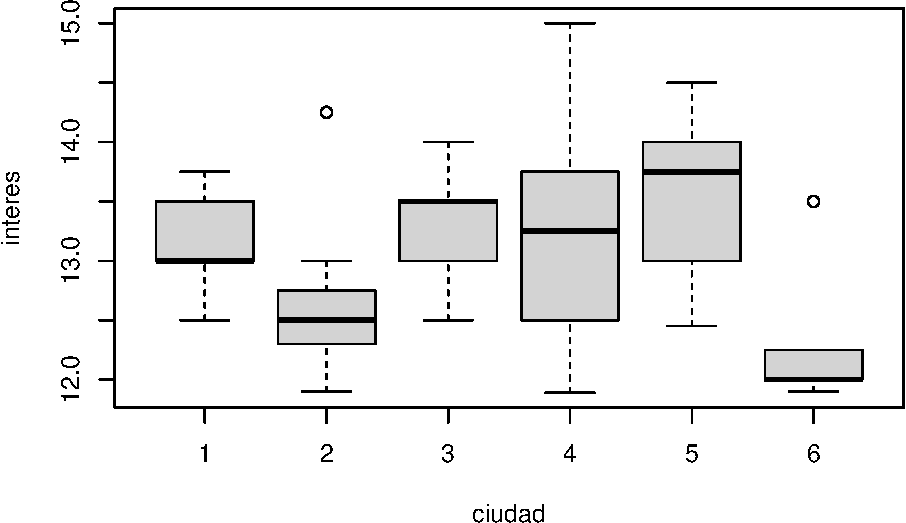
\includegraphics{taller_problemas_resueltos_extra_1_files/figure-latex/unnamed-chunk-20-1.pdf}

Se pide:

\begin{enumerate}
\def\labelenumi{\arabic{enumi}.}
\tightlist
\item
  Comentad el código y el diagrama de caja.
\item
  Se trata de contrastar si hay evidencia de que la tasas medias de
  interés por ciudades son distintas. Definid el ANOVA que contrasta
  esta hipótesis y especificar qué condiciones deben cumplir las
  muestras para poder aplicar el ANOVA.\\
\item
  Comprobad las condiciones del ANOVA con un test KS y un test de Levene
  (con código de \texttt{R}). Justificad las conclusiones.\\
\item
  Realizad el contraste de ANOVA (se cumplan las condiciones o no) y
  redactar adecuadamente la conclusión. Tenéis que hacedlo con funciones
  de \texttt{R}.\\
\item
  Se acepte o no la igualdad de medias realizar las comparaciones dos a
  dos con ajustando los \(p\)-valor tanto por Bonferroni como por Holm
  al nivel de significación \(\alpha=0.1\). Redactad las conclusiones
  que se obtienen de las mismas.
\end{enumerate}

\hypertarget{soluciuxf3n-5}{%
\subsubsection{Solución}\label{soluciuxf3n-5}}

\textbf{Apartado 1}

El código del enunciado nos carga los datos de una web, tenemos que
pasar el parámetro skip=25 para que se salte las 25 primeras lineas del
fichero de texto que son un preámbulo que explica los datos.

En el diagrama de caja vemos que las medias las distribuciones de la
\texttt{Rate} por ciudad son muy distintas, no parecen tener ni medias
ni varianzas iguales

\textbf{Apartado 2}

Las condiciones para realizar un ANOVA son:

\begin{itemize}
\tightlist
\item
  Muestras independientes y aleatorias
\item
  Distribución normal de la Rate \(N(\mu_i,\sigma_i)\) para las seis
  ciudades \(i=1,2,3,4,5,6\).
\item
  homocedasticidad; igualdad de varianzas
  \(\sigma_1=\sigma_2=\sigma_3 =\sigma_4=\sigma_5=\sigma_6.\)
\end{itemize}

El ANOVA que se pide es

\[
\left\{
\begin{array}{ll}
H_0: &  \mu_1=\mu_2=\mu_3=\mu_4=\mu_5=\mu_6\\
H_1: & \mbox{ no  todas las medias son iguales}.
\end{array}
\right.
\]

\textbf{Apartado 3}

El siguiente código realiza un test KS con corrección de Lillie para la
normalidad de la variable Rate en cada una de la seis ciudades

\begin{Shaded}
\begin{Highlighting}[]
\KeywordTok{library}\NormalTok{(nortest)}
\KeywordTok{lillie.test}\NormalTok{(datos\_interes}\OperatorTok{$}\NormalTok{interes[datos\_interes}\OperatorTok{$}\NormalTok{ciudad}\OperatorTok{==}\DecValTok{1}\NormalTok{])}
\end{Highlighting}
\end{Shaded}

\begin{verbatim}
## 
##  Lilliefors (Kolmogorov-Smirnov) normality test
## 
## data:  datos_interes$interes[datos_interes$ciudad == 1]
## D = 0.22384, p-value = 0.2163
\end{verbatim}

\begin{Shaded}
\begin{Highlighting}[]
\KeywordTok{lillie.test}\NormalTok{(datos\_interes}\OperatorTok{$}\NormalTok{interes[datos\_interes}\OperatorTok{$}\NormalTok{ciudad}\OperatorTok{==}\DecValTok{2}\NormalTok{])}
\end{Highlighting}
\end{Shaded}

\begin{verbatim}
## 
##  Lilliefors (Kolmogorov-Smirnov) normality test
## 
## data:  datos_interes$interes[datos_interes$ciudad == 2]
## D = 0.22884, p-value = 0.1903
\end{verbatim}

\begin{Shaded}
\begin{Highlighting}[]
\KeywordTok{lillie.test}\NormalTok{(datos\_interes}\OperatorTok{$}\NormalTok{interes[datos\_interes}\OperatorTok{$}\NormalTok{ciudad}\OperatorTok{==}\DecValTok{3}\NormalTok{])}
\end{Highlighting}
\end{Shaded}

\begin{verbatim}
## 
##  Lilliefors (Kolmogorov-Smirnov) normality test
## 
## data:  datos_interes$interes[datos_interes$ciudad == 3]
## D = 0.19145, p-value = 0.4459
\end{verbatim}

\begin{Shaded}
\begin{Highlighting}[]
\KeywordTok{lillie.test}\NormalTok{(datos\_interes}\OperatorTok{$}\NormalTok{interes[datos\_interes}\OperatorTok{$}\NormalTok{ciudad}\OperatorTok{==}\DecValTok{4}\NormalTok{])}
\end{Highlighting}
\end{Shaded}

\begin{verbatim}
## 
##  Lilliefors (Kolmogorov-Smirnov) normality test
## 
## data:  datos_interes$interes[datos_interes$ciudad == 4]
## D = 0.11264, p-value = 0.9852
\end{verbatim}

\begin{Shaded}
\begin{Highlighting}[]
\KeywordTok{lillie.test}\NormalTok{(datos\_interes}\OperatorTok{$}\NormalTok{interes[datos\_interes}\OperatorTok{$}\NormalTok{ciudad}\OperatorTok{==}\DecValTok{5}\NormalTok{])}
\end{Highlighting}
\end{Shaded}

\begin{verbatim}
## 
##  Lilliefors (Kolmogorov-Smirnov) normality test
## 
## data:  datos_interes$interes[datos_interes$ciudad == 5]
## D = 0.20021, p-value = 0.3743
\end{verbatim}

\begin{Shaded}
\begin{Highlighting}[]
\KeywordTok{lillie.test}\NormalTok{(datos\_interes}\OperatorTok{$}\NormalTok{interes[datos\_interes}\OperatorTok{$}\NormalTok{ciudad}\OperatorTok{==}\DecValTok{6}\NormalTok{])}
\end{Highlighting}
\end{Shaded}

\begin{verbatim}
## 
##  Lilliefors (Kolmogorov-Smirnov) normality test
## 
## data:  datos_interes$interes[datos_interes$ciudad == 6]
## D = 0.3494, p-value = 0.002236
\end{verbatim}

No podemos rechazar la normalidad con el lillie.test en las 5 primeras
ciudades, pero parece que la última está lejos de ser normal.

Ahora comprobemos que

\[
\left\{
\begin{array}{ll}
H_0: &  \sigma^2_1=\sigma^2_2=\sigma^2_3=\sigma^2_4=\sigma^2_5=\sigma^2_6\\
H_1: & \mbox{ no  todas las varianzas son iguales}.
\end{array}
\right.
\]

con el test de Levene (o el de Bartlett)

\begin{Shaded}
\begin{Highlighting}[]
\KeywordTok{library}\NormalTok{(car)}
\KeywordTok{print}\NormalTok{(}\KeywordTok{leveneTest}\NormalTok{(datos\_interes}\OperatorTok{$}\NormalTok{interes}\OperatorTok{\textasciitilde{}}\KeywordTok{as.factor}\NormalTok{(datos\_interes}\OperatorTok{$}\NormalTok{ciudad)))}
\end{Highlighting}
\end{Shaded}

\begin{verbatim}
## Levene's Test for Homogeneity of Variance (center = median)
##       Df F value Pr(>F)
## group  5  1.2797 0.2882
##       48
\end{verbatim}

El test de levene nos da un \(p\)-valor superior a 0.28 aceptamos la
igualdad de varianzas

\textbf{Apartado 4}

Resolvemos el ANOVA con el código siguiente

\begin{Shaded}
\begin{Highlighting}[]
\KeywordTok{summary}\NormalTok{(}\KeywordTok{aov}\NormalTok{(datos\_interes}\OperatorTok{$}\NormalTok{interes}\OperatorTok{\textasciitilde{}}\KeywordTok{as.factor}\NormalTok{(datos\_interes}\OperatorTok{$}\NormalTok{ciudad)))}
\end{Highlighting}
\end{Shaded}

\begin{verbatim}
##                                 Df Sum Sq Mean Sq F value  Pr(>F)   
## as.factor(datos_interes$ciudad)  5  10.95  2.1891   4.829 0.00117 **
## Residuals                       48  21.76  0.4533                   
## ---
## Signif. codes:  0 '***' 0.001 '**' 0.01 '*' 0.05 '.' 0.1 ' ' 1
\end{verbatim}

El \(p\)-valor es muy bajo 0.00117 rechazamos la igualdad de las seis
medias, al menos hay dos distintas.

Comprobamos por gusto el \(p\)-valor a partir de los datos del summary

\begin{Shaded}
\begin{Highlighting}[]
\NormalTok{Fest=}\FloatTok{2.1891}\OperatorTok{/}\FloatTok{0.4533}
\NormalTok{Fest}
\end{Highlighting}
\end{Shaded}

\begin{verbatim}
## [1] 4.829252
\end{verbatim}

\begin{Shaded}
\begin{Highlighting}[]
\DecValTok{1}\OperatorTok{{-}}\KeywordTok{pf}\NormalTok{(Fest,}\DecValTok{5}\NormalTok{,}\DecValTok{48}\NormalTok{)}
\end{Highlighting}
\end{Shaded}

\begin{verbatim}
## [1] 0.001174782
\end{verbatim}

\begin{Shaded}
\begin{Highlighting}[]
\KeywordTok{pf}\NormalTok{(Fest,}\DecValTok{5}\NormalTok{,}\DecValTok{48}\NormalTok{,}\DataTypeTok{lower.tail =} \OtherTok{FALSE}\NormalTok{)}
\end{Highlighting}
\end{Shaded}

\begin{verbatim}
## [1] 0.001174782
\end{verbatim}

\textbf{Apartado 5}

Comparemos las medias dos a dos son 15 comparaciones

\begin{Shaded}
\begin{Highlighting}[]
\KeywordTok{pairwise.t.test}\NormalTok{(datos\_interes}\OperatorTok{$}\NormalTok{interes,}\KeywordTok{as.factor}\NormalTok{(datos\_interes}\OperatorTok{$}\NormalTok{ciudad),}\DataTypeTok{p.adjust.method =} \StringTok{"holm"}\NormalTok{)}
\end{Highlighting}
\end{Shaded}

\begin{verbatim}
## 
##  Pairwise comparisons using t tests with pooled SD 
## 
## data:  datos_interes$interes and as.factor(datos_interes$ciudad) 
## 
##   1      2      3      4      5     
## 2 0.5781 -      -      -      -     
## 3 1.0000 0.3330 -      -      -     
## 4 1.0000 0.4651 1.0000 -      -     
## 5 1.0000 0.0926 1.0000 1.0000 -     
## 6 0.0353 1.0000 0.0148 0.0244 0.0028
## 
## P value adjustment method: holm
\end{verbatim}

Nos piden que decidamos con \(\alpha=0.1\), así que rechazaremos la
igualdad de medias de todas las comparaciones con \(p\)-valor inferior a
\(0.1\).

Tenemos que rechazar la igualdad de medias entre la ciudad 2 con la 5 y
la de la ciudad 6 con las ciudades 1, 3, 4 y 5.

\hypertarget{problema-7-cuestiones-cortas}{%
\subsection{Problema 7: Cuestiones
cortas}\label{problema-7-cuestiones-cortas}}

\begin{itemize}
\tightlist
\item
  Cuestión 1: Supongamos que conocemos el \(p\)-valor de un contraste.
  Para que valores de nivel de significación \(\alpha\) RECHAZAMOS la
  hipótesis nula.
\item
  Cuestión 2: Hemos realizado un ANOVA de un factor con 3 niveles, y
  hemos obtenido un \(p\)-valor de 0.001. Suponiendo que las poblaciones
  satisfacen las condiciones para que el ANOVA tenga sentido, ¿podemos
  afirmar con un nivel de significación \(\alpha= 0.05\) que las medias
  de los tres niveles son diferentes dos a dos? Justificad la respuesta.
\item
  Cuestión 3: Lanzamos 300 veces un dado de 6 caras de parchís, queremos
  contrastar que los resultados son equiprobables. ¿Cuáles serian las
  frecuencias esperadas o teóricas del contraste?
\item
  Cuestión 4: En un ANOVA de una vía, queremos contrastar si los 6
  niveles de un factor definen poblaciones con la misma media. Sabemos
  que estas seis poblaciones son normales con la misma varianza
  \(\sigma=2\). Estudiamos a 11 individuos de cada nivel y obtenemos que
  \(SS_{Total}=256.6\) y \(SS_{Tr}=60.3\). ¿Qué vale \(SS_E\). ¿Qué
  valor estimamos que tiene \(\sigma^2\)?
\item
  Cuestión 5: Calculad la correlación entre los vectores de datos
  \(x=(1,3,4,4)\), \(y=(2,4,12,6)\).
\item
  Cuestión 6: De estas cuatro matrices, indicad cuáles pueden ser
  matrices de correlaciones, y explicad por qué.
\end{itemize}

\(A=\left(\begin{array}{cc} 1 & 0.8\\-0.8 & 1\end{array}\right)\),
\(B=\left(\begin{array}{cc} 0.8 & 0.6\\0.6 & 0.8\end{array}\right)\),
\(C=\left(\begin{array}{cc} 1 & 0\\0 & 1\end{array}\right)\),
\(D=\left(\begin{array}{cc} 1 & 1.2\\1.2 & 1\end{array}\right)\).

\hypertarget{soluciuxf3n-6}{%
\subsubsection{Solución}\label{soluciuxf3n-6}}

\textbf{Cuestion 1}: Rechazamos la hipótesis nula para todos los niveles
de significación \(\alpha\) menores que el \(p\)-valor.

\textbf{Cuestion 2}: No, no podemos afirmar eso. Lo que sabemos después
de rechazar un ANOVA es que hay al menos dos medias distintas.

\textbf{Cuestion 3}: pues son

\begin{Shaded}
\begin{Highlighting}[]
\NormalTok{probs=}\KeywordTok{c}\NormalTok{(}\DecValTok{1}\OperatorTok{/}\DecValTok{6}\NormalTok{,}\DecValTok{1}\OperatorTok{/}\DecValTok{6}\NormalTok{,}\DecValTok{1}\OperatorTok{/}\DecValTok{6}\NormalTok{,}\DecValTok{1}\OperatorTok{/}\DecValTok{6}\NormalTok{,}\DecValTok{1}\OperatorTok{/}\DecValTok{6}\NormalTok{,}\DecValTok{1}\OperatorTok{/}\DecValTok{6}\NormalTok{)}
\NormalTok{frec.esp=}\DecValTok{300}\OperatorTok{*}\NormalTok{probs}
\NormalTok{frec.esp}
\end{Highlighting}
\end{Shaded}

\begin{verbatim}
## [1] 50 50 50 50 50 50
\end{verbatim}

\textbf{Cuestion 4} \$SS\_E=SS\_\{Total\}-SS-\{Tr\}=256.6-60.3=196.3.

El número de observaciones totales es \(N=11\cdot 6=66\) y el número de
niveles del factor es \(k=6\).

El estimador de la varianza conjunto \(\sigma^2\) es
\(MS_E=\frac{SS_e}{N-k}=\frac{196.3}{66-6}=17.8454545.\)

*\textbf{Cuestión 5}

\begin{Shaded}
\begin{Highlighting}[]
\NormalTok{x=}\KeywordTok{c}\NormalTok{(}\DecValTok{1}\NormalTok{,}\DecValTok{3}\NormalTok{,}\DecValTok{4}\NormalTok{,}\DecValTok{4}\NormalTok{)}
\NormalTok{y=}\KeywordTok{c}\NormalTok{(}\DecValTok{2}\NormalTok{,}\DecValTok{4}\NormalTok{,}\DecValTok{12}\NormalTok{,}\DecValTok{6}\NormalTok{)}
\KeywordTok{cor}\NormalTok{(x,y)}
\end{Highlighting}
\end{Shaded}

\begin{verbatim}
## [1] 0.7637626
\end{verbatim}

\textbf{Cuestión 6}

Son matrices de correlaciones 2x2 sabemos que la diagonal tiene que ser
1 pues es la correlación de una variable consigo misma. También sabemos
que \(\rho_{xy}=\rho_{yx}\) así que la matriz debe ser simétrica. Además
\(-1\leq\rho_{xy}\leq. 1\).

\(A\) no es simétrica, \(B\) no tiene la diagonal de unos y \(D\) tienen
valores mayores que 1 luego estas tres matrices no son de correlaciones.
La única matriz que cumple todas las condiciones es la \(C\).

\hypertarget{problema-8-contraste-de-proporciones-de-dos-muestras-independientes.}{%
\subsection{Problema 8: Contraste de proporciones de dos muestras
independientes.}\label{problema-8-contraste-de-proporciones-de-dos-muestras-independientes.}}

Queremos comparar las proporciones de aciertos de dos redes neuronales
que detectan tipos si una foto con un móvil de una avispa es una
\href{https://es.wikipedia.org/wiki/Vespa_velutina}{avispa velutina o
asiática}. Esta avispa en una especie invasora y peligrosa por el veneno
de su picadura. Para ello disponemos de una muestra de 1000 imágenes de
insectos etiquetadas como avispa velutina y no velutina.

\href{http://bioinfo.uib.es/~recerca/MATIIIGINF/velutina}{Aquí tenéis el
acceso a los datos}. Cada uno está en fichero los aciertos están
codificados con 1 y los fallos con 0.

Se pide:

\begin{enumerate}
\def\labelenumi{\arabic{enumi}.}
\tightlist
\item
  Cargad los datos desde el servidos y calcular el tamaño de las
  muestras y la proporción de aciertos de cada muestra.
\item
  Contrastad si hay evidencia de que las las proporciones de aciertos
  del algoritmo 1 son mayores que las del algoritmo 2. Definid bien las
  hipótesis y las condiciones del contraste. Tenéis que hacer el
  contraste con funciones de \texttt{R} y resolver el contrate con el
  \(p\)-valor.
\item
  Calculad e interpretar los intervalos de confianza para la diferencia
  de proporciones asociados al test anterior, con funciones de R.
\end{enumerate}

\hypertarget{soluciuxf3n-7}{%
\subsubsection{Solución}\label{soluciuxf3n-7}}

\begin{Shaded}
\begin{Highlighting}[]
\NormalTok{algoritmo1=}\KeywordTok{read.table}\NormalTok{(}\StringTok{"http://bioinfo.uib.es/\textasciitilde{}recerca/MATIIIGINF/velutina/algoritmo1.csv"}\NormalTok{)}
\NormalTok{algoritmo2=}\KeywordTok{read.table}\NormalTok{(}\StringTok{"http://bioinfo.uib.es/\textasciitilde{}recerca/MATIIIGINF/velutina/algoritmo2.csv"}\NormalTok{)}
\end{Highlighting}
\end{Shaded}

Proporción aciertos de cada algoritmo

\begin{Shaded}
\begin{Highlighting}[]
\NormalTok{n1=}\KeywordTok{dim}\NormalTok{(algoritmo1)[}\DecValTok{1}\NormalTok{]}
\NormalTok{n1}
\end{Highlighting}
\end{Shaded}

\begin{verbatim}
## [1] 500
\end{verbatim}

\begin{Shaded}
\begin{Highlighting}[]
\NormalTok{n1=}\KeywordTok{length}\NormalTok{(algoritmo1}\OperatorTok{$}\NormalTok{V1)}
\NormalTok{n1}
\end{Highlighting}
\end{Shaded}

\begin{verbatim}
## [1] 500
\end{verbatim}

\begin{Shaded}
\begin{Highlighting}[]
\NormalTok{n2=}\KeywordTok{length}\NormalTok{(algoritmo2}\OperatorTok{$}\NormalTok{V1)}
\NormalTok{n2}
\end{Highlighting}
\end{Shaded}

\begin{verbatim}
## [1] 500
\end{verbatim}

\begin{Shaded}
\begin{Highlighting}[]
\NormalTok{aciertos\_absolutos\_algoritmo1=}\KeywordTok{table}\NormalTok{(algoritmo1)[}\StringTok{"1"}\NormalTok{]}
\NormalTok{aciertos\_absolutos\_algoritmo1}
\end{Highlighting}
\end{Shaded}

\begin{verbatim}
##   1 
## 396
\end{verbatim}

\begin{Shaded}
\begin{Highlighting}[]
\NormalTok{p1=}\KeywordTok{prop.table}\NormalTok{(}\KeywordTok{table}\NormalTok{(algoritmo1))[}\StringTok{"1"}\NormalTok{]}
\NormalTok{p1}
\end{Highlighting}
\end{Shaded}

\begin{verbatim}
##     1 
## 0.792
\end{verbatim}

\begin{Shaded}
\begin{Highlighting}[]
\NormalTok{aciertos\_absolutos\_algoritmo2=}\KeywordTok{table}\NormalTok{(algoritmo2)[}\StringTok{"1"}\NormalTok{]}
\NormalTok{aciertos\_absolutos\_algoritmo2}
\end{Highlighting}
\end{Shaded}

\begin{verbatim}
##   1 
## 437
\end{verbatim}

\begin{Shaded}
\begin{Highlighting}[]
\NormalTok{p2=}\KeywordTok{prop.table}\NormalTok{(}\KeywordTok{table}\NormalTok{(algoritmo2))[}\StringTok{"1"}\NormalTok{]}
\NormalTok{p2}
\end{Highlighting}
\end{Shaded}

\begin{verbatim}
##     1 
## 0.874
\end{verbatim}

Después de los cálculos preliminares si denotamos las proporciones
poblacionales de aciertos de cada algoritmo por \(p_1\) y \(p_2\)
respectivamente, el contraste que nos piden es

\[
\left\{
\begin{array}{ll}
H_0: & p_1=p_2\\
H_1: & p_1>p_2\\
\end{array}
\right.
\]

estamos ante un diseño de comparación de proporciones con muestras
independientes. Con R lo podemos resolver con el \texttt{fisher.test} o
con el \texttt{prop.test}

\begin{Shaded}
\begin{Highlighting}[]
\NormalTok{x=}\KeywordTok{matrix}\NormalTok{(}\KeywordTok{c}\NormalTok{(aciertos\_absolutos\_algoritmo1,n1}\OperatorTok{{-}}\NormalTok{aciertos\_absolutos\_algoritmo1,}
\NormalTok{           aciertos\_absolutos\_algoritmo2,n2}\OperatorTok{{-}}\NormalTok{aciertos\_absolutos\_algoritmo2),}
         \DataTypeTok{ncol=}\DecValTok{2}\NormalTok{,}\DataTypeTok{byrow=}\OtherTok{FALSE}\NormalTok{)}
\NormalTok{x}
\end{Highlighting}
\end{Shaded}

\begin{verbatim}
##      [,1] [,2]
## [1,]  396  437
## [2,]  104   63
\end{verbatim}

\begin{Shaded}
\begin{Highlighting}[]
\KeywordTok{fisher.test}\NormalTok{(x,}\DataTypeTok{alternative=}\StringTok{"greater"}\NormalTok{,}\DataTypeTok{conf.level=}\FloatTok{0.95}\NormalTok{)}
\end{Highlighting}
\end{Shaded}

\begin{verbatim}
## 
##  Fisher's Exact Test for Count Data
## 
## data:  x
## p-value = 0.9998
## alternative hypothesis: true odds ratio is greater than 1
## 95 percent confidence interval:
##  0.4056457       Inf
## sample estimates:
## odds ratio 
##  0.5492712
\end{verbatim}

\begin{Shaded}
\begin{Highlighting}[]
\KeywordTok{c}\NormalTok{(aciertos\_absolutos\_algoritmo1,aciertos\_absolutos\_algoritmo2)}
\end{Highlighting}
\end{Shaded}

\begin{verbatim}
##   1   1 
## 396 437
\end{verbatim}

\begin{Shaded}
\begin{Highlighting}[]
\KeywordTok{c}\NormalTok{(n1,n2)}
\end{Highlighting}
\end{Shaded}

\begin{verbatim}
## [1] 500 500
\end{verbatim}

\begin{Shaded}
\begin{Highlighting}[]
\KeywordTok{prop.test}\NormalTok{(}\KeywordTok{c}\NormalTok{(aciertos\_absolutos\_algoritmo1,aciertos\_absolutos\_algoritmo2), }\KeywordTok{c}\NormalTok{(n1,n2),}\DataTypeTok{alternative=}\StringTok{"greater"}\NormalTok{,}\DataTypeTok{conf.level=}\FloatTok{0.95}\NormalTok{)}
\end{Highlighting}
\end{Shaded}

\begin{verbatim}
## 
##  2-sample test for equality of proportions with continuity correction
## 
## data:  c(aciertos_absolutos_algoritmo1, aciertos_absolutos_algoritmo2) out of c(n1, n2)
## X-squared = 11.502, df = 1, p-value = 0.9997
## alternative hypothesis: greater
## 95 percent confidence interval:
##  -0.1225654  1.0000000
## sample estimates:
## prop 1 prop 2 
##  0.792  0.874
\end{verbatim}

Con ambos test obtenemos \(p\) valores altos (el más pequeño es el de
Fisher y es mayor que \(0.4\), así que no podemos rechazar que las
proporciones de aciertos de los dos algoritmos sean iguales contra que
la proporción de aciertos del algoritmo 1 es mejor que la del 2.

El intervalo de confianza asociado a este test es

\begin{Shaded}
\begin{Highlighting}[]
\KeywordTok{prop.test}\NormalTok{(}\KeywordTok{c}\NormalTok{(aciertos\_absolutos\_algoritmo1,aciertos\_absolutos\_algoritmo2), }\KeywordTok{c}\NormalTok{(n1,n2),}\DataTypeTok{alternative=}\StringTok{"greater"}\NormalTok{,}\DataTypeTok{conf.level=}\FloatTok{0.95}\NormalTok{)}\OperatorTok{$}\NormalTok{conf.int}
\end{Highlighting}
\end{Shaded}

\begin{verbatim}
## [1] -0.1225654  1.0000000
## attr(,"conf.level")
## [1] 0.95
\end{verbatim}

luego con una probabilidad del 95\% la \(p_1-p_2> -1\) contiene el 0 y
no podemos despreciar que sean iguales contra que \(p_1>p_2.\)

\hypertarget{problema-9-contraste-de-proporciones-de-dos-muestras-emparejadas.}{%
\subsection{Problema 9 : Contraste de proporciones de dos muestras
emparejadas.}\label{problema-9-contraste-de-proporciones-de-dos-muestras-emparejadas.}}

En el problema anterior hemos decidido quedarnos con el mejor de los
algoritmos y mejorarlo. Pasamos las mismas 1000 imágenes a la
version\_beta del algoritmo y a la version\_alpha.
\href{http://bioinfo.uib.es/~recerca/MATIIIGINF/velutina2}{Aquí tenéis
el acceso a los datos en el mismo orden para las 1000 imágenes}. Cada
uno está en fichero los aciertos están codificados con 1 y los fallos
con 0.

\begin{enumerate}
\def\labelenumi{\arabic{enumi}.}
\tightlist
\item
  Cargad los datos desde el servidos y calcular el tamaño de las
  muestras y la proporción de aciertos de cada muestra.
\item
  Contrastad si hay evidencia de que las las proporciones de aciertos
  del algoritmo alfa son iguales que las del algoritmo beta. Definid
  bien las hipótesis y las condiciones del contraste. Tenéis que hacer
  el contraste con funciones de \texttt{R} y resolver el contrate con el
  \(p\)-valor.
\end{enumerate}

\hypertarget{soluciuxf3n-8}{%
\subsubsection{Solución}\label{soluciuxf3n-8}}

Cargamos los datos y hacemos los cálculos preliminares

\begin{Shaded}
\begin{Highlighting}[]
\NormalTok{algoritmoalfa=}\KeywordTok{read.table}\NormalTok{(}\StringTok{"http://bioinfo.uib.es/\textasciitilde{}recerca/MATIIIGINF/velutina2/algoritmo\_alpha.csv"}\NormalTok{)}
\NormalTok{algoritmobeta=}\KeywordTok{read.table}\NormalTok{(}\StringTok{"http://bioinfo.uib.es/\textasciitilde{}recerca/MATIIIGINF/velutina2/algoritmo\_beta.csv"}\NormalTok{)}
\end{Highlighting}
\end{Shaded}

El test que nos piden es

\[
\left\{
\begin{array}{ll}
H_0: & p_{\alpha}=p_{\beta}\\
H_1: & p_{\alpha}\not=p_{\beta}\\
\end{array}
\right.
\]

Es un diseño de muestras emparejadas y tenemos que utilizar el
\texttt{mcnear.test}:

\begin{Shaded}
\begin{Highlighting}[]
\NormalTok{X=}\KeywordTok{table}\NormalTok{(algoritmoalfa}\OperatorTok{$}\NormalTok{V1,algoritmobeta}\OperatorTok{$}\NormalTok{V1)}
\NormalTok{X}
\end{Highlighting}
\end{Shaded}

\begin{verbatim}
##    
##       0   1
##   0  15 110
##   1  88 787
\end{verbatim}

\begin{Shaded}
\begin{Highlighting}[]
\KeywordTok{mcnemar.test}\NormalTok{(X)}
\end{Highlighting}
\end{Shaded}

\begin{verbatim}
## 
##  McNemar's Chi-squared test with continuity correction
## 
## data:  X
## McNemar's chi-squared = 2.2273, df = 1, p-value = 0.1356
\end{verbatim}

El \(p\)-valor es 0.1356 no podemos rechazar la igualdad de la
proporción de aciertos.

\hypertarget{problema-10-anova-comparaciuxf3n-media-puntuaciones-seguxfan-fabricante.}{%
\subsection{Problema 10 : ANOVA comparación media puntuaciones según
fabricante.}\label{problema-10-anova-comparaciuxf3n-media-puntuaciones-seguxfan-fabricante.}}

Una vez mejorado nuestro algoritmo queremos saber su comportamiento bajo
distintos tipos de móviles.

Seleccionamos 6 móviles de la misma gama de calidad de 6 fabricantes
distintos. A los fabricantes los denotamos por F1, F2, F3, F4, F5 y F6.

Vamos a jugar no con la clasificación sino con el score que produce el
algoritmo. Para ello seleccionamos 4 muestra aleatorias de fotos de
insectos enviadas por los usuarios y la puntuación (\emph{score}) que
nos da el algoritmo que es una variable aleatoria continua de con rango
de 0 a 100.

La idea es comprobar si la media de las puntuaciones del algoritmo es la
misma para cada uno de los fabricantes.

Los datos los podéis descargar de esta dirección del
\href{http://bioinfo.uib.es/~recerca/MATIIIGINF/anova_score/}{servidor
bioinfo.uib.es}.

Antes de descargarlo, visualizar el fichero desde el navegador, para
saber cómo descargarlo.

\begin{enumerate}
\def\labelenumi{\arabic{enumi}.}
\tightlist
\item
  ¿Podemos asegurar que la muestras son normales en cada grupo? ¿y son
  homocedásticas? Justificar la respuesta con el correspondiente código
  en R comentado.
\item
  Escribid formalmente la hipótesis nula y la alternativa. Calcular la
  tabla de ANOVA y resuelve el test de forma manual.
\item
  Calcular la tabla de ANOVA y resuelve el test con la función
  \texttt{aov} de R.
\item
  Haced una comparación de pares con la función adecuada de R para la
  corrección del holm al nivel de significación \(\alpha=0.1\).
  Interpreta el resultado.
\item
  Comparar por grupos con el test de Duncan del paquete
  \texttt{agricolae}. Interpreta el resultado.
\end{enumerate}

\hypertarget{soluciuxf3n-9}{%
\subsubsection{Solución}\label{soluciuxf3n-9}}

\begin{Shaded}
\begin{Highlighting}[]
\NormalTok{df=}\KeywordTok{read.table}\NormalTok{(}\StringTok{"http://bioinfo.uib.es/\textasciitilde{}recerca/MATIIIGINF/anova\_score/score\_manufacturer.csv"}\NormalTok{)}
\KeywordTok{head}\NormalTok{(df)}
\end{Highlighting}
\end{Shaded}

\begin{verbatim}
##      score manufacturer
## 1 69.32030           F1
## 2 66.93433           F1
## 3 67.70541           F1
## 4 63.47195           F1
## 5 65.58738           F1
## 6 65.47437           F1
\end{verbatim}

\begin{Shaded}
\begin{Highlighting}[]
\NormalTok{df}\OperatorTok{$}\NormalTok{manufacturer=}\KeywordTok{as.factor}\NormalTok{(df}\OperatorTok{$}\NormalTok{manufacturer)}
\end{Highlighting}
\end{Shaded}

\begin{Shaded}
\begin{Highlighting}[]
\KeywordTok{table}\NormalTok{(df}\OperatorTok{$}\NormalTok{manufacturer)}
\end{Highlighting}
\end{Shaded}

\begin{verbatim}
## 
##  F1  F2  F3  F4  F5  F6 
## 100 100 100 100 100 100
\end{verbatim}

Tenemos que comprobar la normalidad de la distribución de la muestra
para cada nivel del factor \(i=1,2,3,4,5,6\); el test es

\[
\left\{
\begin{array}{ll}
H_0: & \mbox{la distribución de los datos  en el nivel $F_i$ es normal,}\\
H_1: & \mbox{la distribución de los datos en el nivel $F_i$ no es normal,}\\
\end{array}
\right.
\]

\begin{Shaded}
\begin{Highlighting}[]
\KeywordTok{library}\NormalTok{(nortest)}
\CommentTok{\# El test KS\_Lillie para en nivel "F1"}
\CommentTok{\#lillie.test(df$score[df$manufacturer=="F1"])}
\KeywordTok{sapply}\NormalTok{(}\KeywordTok{levels}\NormalTok{(df}\OperatorTok{$}\NormalTok{manufacturer), }\DataTypeTok{FUN=}\ControlFlowTok{function}\NormalTok{(x) \{}\KeywordTok{print}\NormalTok{(}\KeywordTok{lillie.test}\NormalTok{(df}\OperatorTok{$}\NormalTok{score[df}\OperatorTok{$}\NormalTok{manufacturer}\OperatorTok{==}\NormalTok{x]))\})}
\end{Highlighting}
\end{Shaded}

\begin{verbatim}
## 
##  Lilliefors (Kolmogorov-Smirnov) normality test
## 
## data:  df$score[df$manufacturer == x]
## D = 0.091505, p-value = 0.03825
## 
## 
##  Lilliefors (Kolmogorov-Smirnov) normality test
## 
## data:  df$score[df$manufacturer == x]
## D = 0.067758, p-value = 0.3121
## 
## 
##  Lilliefors (Kolmogorov-Smirnov) normality test
## 
## data:  df$score[df$manufacturer == x]
## D = 0.069567, p-value = 0.2744
## 
## 
##  Lilliefors (Kolmogorov-Smirnov) normality test
## 
## data:  df$score[df$manufacturer == x]
## D = 0.069567, p-value = 0.2744
## 
## 
##  Lilliefors (Kolmogorov-Smirnov) normality test
## 
## data:  df$score[df$manufacturer == x]
## D = 0.069567, p-value = 0.2744
## 
## 
##  Lilliefors (Kolmogorov-Smirnov) normality test
## 
## data:  df$score[df$manufacturer == x]
## D = 0.10632, p-value = 0.007255
\end{verbatim}

\begin{verbatim}
##           F1                                              
## statistic 0.09150477                                      
## p.value   0.03825059                                      
## method    "Lilliefors (Kolmogorov-Smirnov) normality test"
## data.name "df$score[df$manufacturer == x]"                
##           F2                                              
## statistic 0.06775771                                      
## p.value   0.3121052                                       
## method    "Lilliefors (Kolmogorov-Smirnov) normality test"
## data.name "df$score[df$manufacturer == x]"                
##           F3                                              
## statistic 0.06956719                                      
## p.value   0.2743622                                       
## method    "Lilliefors (Kolmogorov-Smirnov) normality test"
## data.name "df$score[df$manufacturer == x]"                
##           F4                                              
## statistic 0.06956719                                      
## p.value   0.2743622                                       
## method    "Lilliefors (Kolmogorov-Smirnov) normality test"
## data.name "df$score[df$manufacturer == x]"                
##           F5                                              
## statistic 0.06956719                                      
## p.value   0.2743622                                       
## method    "Lilliefors (Kolmogorov-Smirnov) normality test"
## data.name "df$score[df$manufacturer == x]"                
##           F6                                              
## statistic 0.1063201                                       
## p.value   0.007255259                                     
## method    "Lilliefors (Kolmogorov-Smirnov) normality test"
## data.name "df$score[df$manufacturer == x]"
\end{verbatim}

\begin{Shaded}
\begin{Highlighting}[]
\CommentTok{\# También podemos hacer un bucle clásico}
\CommentTok{\#for(Fabricante in levels(df$manufacturer))\{}
\CommentTok{\#print(lillie.test(df$score[df$manufacturer==Fabricante]))}
\CommentTok{\#\}}
\end{Highlighting}
\end{Shaded}

El nivel ``F1'' y ``F6'' dan valores pequeños no podemos asegurar la
normalidad en estos casos.

Nos aseguramos con el ómnibus test de D'Agostino

\begin{Shaded}
\begin{Highlighting}[]
\KeywordTok{library}\NormalTok{(fBasics)}
\end{Highlighting}
\end{Shaded}

\begin{verbatim}
## Loading required package: timeDate
\end{verbatim}

\begin{verbatim}
## Loading required package: timeSeries
\end{verbatim}

\begin{verbatim}
## 
## Attaching package: 'fBasics'
\end{verbatim}

\begin{verbatim}
## The following object is masked from 'package:car':
## 
##     densityPlot
\end{verbatim}

\begin{Shaded}
\begin{Highlighting}[]
\KeywordTok{dagoTest}\NormalTok{(df}\OperatorTok{$}\NormalTok{score[df}\OperatorTok{$}\NormalTok{manufacturer}\OperatorTok{==}\StringTok{"F1"}\NormalTok{])}
\end{Highlighting}
\end{Shaded}

\begin{verbatim}
## 
## Title:
##  D'Agostino Normality Test
## 
## Test Results:
##   STATISTIC:
##     Chi2 | Omnibus: 5.8827
##     Z3  | Skewness: 2.1113
##     Z4  | Kurtosis: 1.1939
##   P VALUE:
##     Omnibus  Test: 0.05279 
##     Skewness Test: 0.03475 
##     Kurtosis Test: 0.2325 
## 
## Description:
##  Fri May 21 10:32:33 2021 by user: t169
\end{verbatim}

\begin{Shaded}
\begin{Highlighting}[]
\KeywordTok{dagoTest}\NormalTok{(df}\OperatorTok{$}\NormalTok{score[df}\OperatorTok{$}\NormalTok{manufacturer}\OperatorTok{==}\StringTok{"F6"}\NormalTok{])}
\end{Highlighting}
\end{Shaded}

\begin{verbatim}
## 
## Title:
##  D'Agostino Normality Test
## 
## Test Results:
##   STATISTIC:
##     Chi2 | Omnibus: 1.7625
##     Z3  | Skewness: -1.2831
##     Z4  | Kurtosis: 0.3408
##   P VALUE:
##     Omnibus  Test: 0.4143 
##     Skewness Test: 0.1995 
##     Kurtosis Test: 0.7333 
## 
## Description:
##  Fri May 21 10:32:33 2021 by user: t169
\end{verbatim}

Parece que no podemos rechazar la normalidad para los casos dudosos.

Ahora realizamos el test de comparación de medias \(\mu_i\) para
\(i=1,2,3,4,5,6\) son las medias para cada nivel del factor.

\[
\left\{
\begin{array}{ll}
H_0: & \mu_1=\mu_2=\mu_3=\mu_4=\mu_5=\mu_6\\
H_1: & \mbox{no todas la medias son iguales,}\\
\end{array}
\right.
\]

\begin{Shaded}
\begin{Highlighting}[]
\KeywordTok{summary}\NormalTok{(}\KeywordTok{aov}\NormalTok{(df}\OperatorTok{$}\NormalTok{score}\OperatorTok{\textasciitilde{}}\NormalTok{df}\OperatorTok{$}\NormalTok{manufacturer))}
\end{Highlighting}
\end{Shaded}

\begin{verbatim}
##                  Df Sum Sq Mean Sq F value               Pr(>F)    
## df$manufacturer   5   9143  1828.5   17.54 0.000000000000000317 ***
## Residuals       594  61910   104.2                                 
## ---
## Signif. codes:  0 '***' 0.001 '**' 0.01 '*' 0.05 '.' 0.1 ' ' 1
\end{verbatim}

Como el \(p\)-valor es muy pequeño NO podemos aceptar que las 6 medias
sean iguales

Ahora tenemos que contrastar que pares de medias dos a dos son iguales y
ajustar los \(p\)-valores con el ajuste del \(p\)-valor por el método de
Holm

\begin{Shaded}
\begin{Highlighting}[]
\KeywordTok{pairwise.t.test}\NormalTok{(df}\OperatorTok{$}\NormalTok{score,df}\OperatorTok{$}\NormalTok{manufacturer,}\DataTypeTok{p.adjust.method =} \StringTok{"holm"}\NormalTok{)}
\end{Highlighting}
\end{Shaded}

\begin{verbatim}
## 
##  Pairwise comparisons using t tests with pooled SD 
## 
## data:  df$score and df$manufacturer 
## 
##    F1      F2            F3            F4      F5     
## F2 1.00000 -             -             -       -      
## F3 0.07729 0.44250       -             -       -      
## F4 0.00011 0.00000297115 0.00000000017 -       -      
## F5 0.00011 0.00000297115 0.00000000017 1.00000 -      
## F6 0.00724 0.00040       0.00000014687 1.00000 1.00000
## 
## P value adjustment method: holm
\end{verbatim}

Comparamos los \(p\)-valores con \(0.05\) y aceptamos que las medias de
los niveles \(F_4\), \(F_6\) y \(F_5\) son iguales dos a dos, también
son iguales la media del \(F_1\) con el \(F_2\), y la media del nivel
\(F_2\) con el \(F_3\). EL resto de comparaciones tienen \(p\)-valores
bajos así que no podemos aceptar la igualdad de medias.

Ahora comparamos las medias por grupos de igualdades con el test de
Duncan

\begin{Shaded}
\begin{Highlighting}[]
\KeywordTok{library}\NormalTok{(agricolae)}
\end{Highlighting}
\end{Shaded}

\begin{verbatim}
## 
## Attaching package: 'agricolae'
\end{verbatim}

\begin{verbatim}
## The following objects are masked from 'package:timeDate':
## 
##     kurtosis, skewness
\end{verbatim}

\begin{Shaded}
\begin{Highlighting}[]
\NormalTok{resultado.anova=}\KeywordTok{aov}\NormalTok{(df}\OperatorTok{$}\NormalTok{score}\OperatorTok{\textasciitilde{}}\NormalTok{df}\OperatorTok{$}\NormalTok{manufacturer)}
\KeywordTok{duncan.test}\NormalTok{(resultado.anova,}\StringTok{"df$manufacturer"}\NormalTok{,}\DataTypeTok{group=}\OtherTok{TRUE}\NormalTok{)}\OperatorTok{$}\NormalTok{group}
\end{Highlighting}
\end{Shaded}

\begin{verbatim}
##    df$score groups
## F3 74.07499      a
## F2 71.61166     ab
## F1 70.47337      b
## F6 65.71299      c
## F4 64.07499      c
## F5 64.07499      c
\end{verbatim}

Obtenemos tres grupos el \textbf{a} dice la media de \(\mu_3=mu_2\) el
\textbf{b} dice que \(\mu_2=\mu_1\) y el \textbf{c} dice que
\(\mu_6=\mu_4=\mu_5\). Obtenemos conclusiones similares al test de
comparación de medias.

\hypertarget{problema-11-regresiuxf3n-lineal-simple.}{%
\subsection{Problema 11: Regresión lineal
simple.}\label{problema-11-regresiuxf3n-lineal-simple.}}

Consideremos los siguientes datos

\begin{Shaded}
\begin{Highlighting}[]
\NormalTok{x=}\KeywordTok{c}\NormalTok{(}\OperatorTok{{-}}\DecValTok{2}\NormalTok{,}\OperatorTok{{-}}\DecValTok{1}\NormalTok{,}\DecValTok{2}\NormalTok{,}\DecValTok{0}\NormalTok{,}\DecValTok{1}\NormalTok{,}\DecValTok{2}\NormalTok{)}
\NormalTok{y=}\KeywordTok{c}\NormalTok{(}\OperatorTok{{-}}\DecValTok{7}\NormalTok{, }\DecValTok{{-}5}\NormalTok{,  }\DecValTok{5}\NormalTok{, }\DecValTok{{-}3}\NormalTok{,  }\FloatTok{3.0}\NormalTok{,  }\DecValTok{4}\NormalTok{)}
\KeywordTok{summary}\NormalTok{(}\KeywordTok{lm}\NormalTok{(y}\OperatorTok{\textasciitilde{}}\NormalTok{x))}
\end{Highlighting}
\end{Shaded}

\begin{verbatim}
## 
## Call:
## lm(formula = y ~ x)
## 
## Residuals:
##      1      2      3      4      5      6 
##  0.675 -0.400  0.375 -1.475  1.450 -0.625 
## 
## Coefficients:
##             Estimate Std. Error t value Pr(>|t|)    
## (Intercept)  -1.5250     0.4872  -3.130 0.035176 *  
## x             3.0750     0.3189   9.642 0.000647 ***
## ---
## Signif. codes:  0 '***' 0.001 '**' 0.01 '*' 0.05 '.' 0.1 ' ' 1
## 
## Residual standard error: 1.165 on 4 degrees of freedom
## Multiple R-squared:  0.9587, Adjusted R-squared:  0.9484 
## F-statistic: 92.96 on 1 and 4 DF,  p-value: 0.0006472
\end{verbatim}

\begin{enumerate}
\def\labelenumi{\arabic{enumi}.}
\tightlist
\item
  Calcular manualmente los coeficiente de la regresión lineal de y sobre
  x
\item
  Calcular los valores \(\hat{y}_i=b_0+b_1\cdot x_1\) para los valores
  de la muestra y el error cometido.
\item
  Calcular la estimación de la varianza del error.
\item
  Resolver manualmente el contraste
  \(\left\{\begin{array}{ll} H_0: & \beta_1=0 \\ H_1: & \beta_1\not=0\end{array}\right. ,\)
  calculando el \(p\)-valor.
\item
  Calcular \(SST\), \(SSR\) y \(SSE\).
\item
  Calcular el coeficiente de regresión lineal \(r_{xy}\) y el
  coeficiente de determinación \(R^2\). Interpretad el resultado en
  términos de la cantidad de varianza explicada por el modelo
\item
  Comprobar que los resultados son los mismos que los obtenidos con la
  función \texttt{summary(lm(y\textasciitilde{}x))}.
\end{enumerate}

\hypertarget{soluciuxf3n-10}{%
\subsubsection{Solución}\label{soluciuxf3n-10}}

Faltan añadir los NECESARIOS COMENTARIOS.

\begin{Shaded}
\begin{Highlighting}[]
\NormalTok{x=}\KeywordTok{c}\NormalTok{(}\OperatorTok{{-}}\DecValTok{2}\NormalTok{,}\OperatorTok{{-}}\DecValTok{1}\NormalTok{,}\DecValTok{2}\NormalTok{,}\DecValTok{0}\NormalTok{,}\DecValTok{1}\NormalTok{,}\DecValTok{2}\NormalTok{)}
\NormalTok{y=}\KeywordTok{c}\NormalTok{(}\OperatorTok{{-}}\DecValTok{7}\NormalTok{, }\DecValTok{{-}5}\NormalTok{,  }\DecValTok{5}\NormalTok{, }\DecValTok{{-}3}\NormalTok{,  }\FloatTok{3.0}\NormalTok{,  }\DecValTok{4}\NormalTok{)}
\NormalTok{sol\_lm=}\KeywordTok{lm}\NormalTok{(y}\OperatorTok{\textasciitilde{}}\NormalTok{x)}
\KeywordTok{summary}\NormalTok{(sol\_lm)}
\end{Highlighting}
\end{Shaded}

\begin{verbatim}
## 
## Call:
## lm(formula = y ~ x)
## 
## Residuals:
##      1      2      3      4      5      6 
##  0.675 -0.400  0.375 -1.475  1.450 -0.625 
## 
## Coefficients:
##             Estimate Std. Error t value Pr(>|t|)    
## (Intercept)  -1.5250     0.4872  -3.130 0.035176 *  
## x             3.0750     0.3189   9.642 0.000647 ***
## ---
## Signif. codes:  0 '***' 0.001 '**' 0.01 '*' 0.05 '.' 0.1 ' ' 1
## 
## Residual standard error: 1.165 on 4 degrees of freedom
## Multiple R-squared:  0.9587, Adjusted R-squared:  0.9484 
## F-statistic: 92.96 on 1 and 4 DF,  p-value: 0.0006472
\end{verbatim}

\begin{Shaded}
\begin{Highlighting}[]
\NormalTok{mediay=}\KeywordTok{mean}\NormalTok{(y)}
\NormalTok{mediax=}\KeywordTok{mean}\NormalTok{(x)}
\NormalTok{sdx=}\KeywordTok{sd}\NormalTok{(x)}
\NormalTok{sdy=}\KeywordTok{sd}\NormalTok{(y)}
\NormalTok{sxy=}\KeywordTok{cov}\NormalTok{(x,y)}
\NormalTok{b1=sxy}\OperatorTok{/}\NormalTok{sdx}\OperatorTok{\^{}}\DecValTok{2}
\NormalTok{b1}
\end{Highlighting}
\end{Shaded}

\begin{verbatim}
## [1] 3.075
\end{verbatim}

\begin{Shaded}
\begin{Highlighting}[]
\NormalTok{b0=mediay}\OperatorTok{{-}}\NormalTok{b1}\OperatorTok{*}\NormalTok{mediax}
\NormalTok{b0}
\end{Highlighting}
\end{Shaded}

\begin{verbatim}
## [1] -1.525
\end{verbatim}

\begin{Shaded}
\begin{Highlighting}[]
\NormalTok{sol\_lm}\OperatorTok{$}\NormalTok{coefficients}
\end{Highlighting}
\end{Shaded}

\begin{verbatim}
## (Intercept)           x 
##      -1.525       3.075
\end{verbatim}

\begin{Shaded}
\begin{Highlighting}[]
\KeywordTok{c}\NormalTok{(b0,b1)}\OperatorTok{==}\NormalTok{sol\_lm}\OperatorTok{$}\NormalTok{coefficients}\CommentTok{\# dan distintos errores de redondeo}
\end{Highlighting}
\end{Shaded}

\begin{verbatim}
## (Intercept)           x 
##       FALSE        TRUE
\end{verbatim}

\begin{Shaded}
\begin{Highlighting}[]
\KeywordTok{near}\NormalTok{(}\KeywordTok{c}\NormalTok{(b0,b1),sol\_lm}\OperatorTok{$}\NormalTok{coefficients)}\CommentTok{\# opcional}
\end{Highlighting}
\end{Shaded}

\begin{verbatim}
## (Intercept)           x 
##        TRUE        TRUE
\end{verbatim}

\begin{Shaded}
\begin{Highlighting}[]
\NormalTok{sol\_lm}\OperatorTok{$}\NormalTok{fitted.values}
\end{Highlighting}
\end{Shaded}

\begin{verbatim}
##      1      2      3      4      5      6 
## -7.675 -4.600  4.625 -1.525  1.550  4.625
\end{verbatim}

\begin{Shaded}
\begin{Highlighting}[]
\NormalTok{recta=}\ControlFlowTok{function}\NormalTok{(x) b0}\OperatorTok{+}\NormalTok{b1}\OperatorTok{*}\NormalTok{x}
\NormalTok{y\_est=}\KeywordTok{recta}\NormalTok{(x)}
\NormalTok{y\_est}
\end{Highlighting}
\end{Shaded}

\begin{verbatim}
## [1] -7.675 -4.600  4.625 -1.525  1.550  4.625
\end{verbatim}

\begin{Shaded}
\begin{Highlighting}[]
\KeywordTok{predict}\NormalTok{(sol\_lm,}\DataTypeTok{newdata =} \KeywordTok{data.frame}\NormalTok{(}\DataTypeTok{x=}\NormalTok{x))}
\end{Highlighting}
\end{Shaded}

\begin{verbatim}
##      1      2      3      4      5      6 
## -7.675 -4.600  4.625 -1.525  1.550  4.625
\end{verbatim}

\begin{Shaded}
\begin{Highlighting}[]
\NormalTok{y}
\end{Highlighting}
\end{Shaded}

\begin{verbatim}
## [1] -7 -5  5 -3  3  4
\end{verbatim}

\begin{Shaded}
\begin{Highlighting}[]
\NormalTok{y\_est}
\end{Highlighting}
\end{Shaded}

\begin{verbatim}
## [1] -7.675 -4.600  4.625 -1.525  1.550  4.625
\end{verbatim}

\begin{Shaded}
\begin{Highlighting}[]
\NormalTok{e=y}\OperatorTok{{-}}\NormalTok{y\_est}
\NormalTok{e}
\end{Highlighting}
\end{Shaded}

\begin{verbatim}
## [1]  0.675 -0.400  0.375 -1.475  1.450 -0.625
\end{verbatim}

\begin{Shaded}
\begin{Highlighting}[]
\NormalTok{sol\_lm}\OperatorTok{$}\NormalTok{residuals}
\end{Highlighting}
\end{Shaded}

\begin{verbatim}
##      1      2      3      4      5      6 
##  0.675 -0.400  0.375 -1.475  1.450 -0.625
\end{verbatim}

\begin{Shaded}
\begin{Highlighting}[]
\KeywordTok{mean}\NormalTok{(e) }\CommentTok{\# es cero, pero por error de redondeo no da exacto.}
\end{Highlighting}
\end{Shaded}

\begin{verbatim}
## [1] -0.0000000000000002220446
\end{verbatim}

\begin{Shaded}
\begin{Highlighting}[]
\NormalTok{SSE=}\KeywordTok{sum}\NormalTok{(e}\OperatorTok{\^{}}\DecValTok{2}\NormalTok{)}
\NormalTok{SSE}
\end{Highlighting}
\end{Shaded}

\begin{verbatim}
## [1] 5.425
\end{verbatim}

\begin{Shaded}
\begin{Highlighting}[]
\NormalTok{n=}\KeywordTok{length}\NormalTok{(x)}
\NormalTok{n}
\end{Highlighting}
\end{Shaded}

\begin{verbatim}
## [1] 6
\end{verbatim}

\begin{Shaded}
\begin{Highlighting}[]
\NormalTok{S2=SSE}\OperatorTok{/}\NormalTok{(n}\DecValTok{{-}2}\NormalTok{)}\CommentTok{\#estimacion\_var\_error}
\NormalTok{S2}
\end{Highlighting}
\end{Shaded}

\begin{verbatim}
## [1] 1.35625
\end{verbatim}

\begin{Shaded}
\begin{Highlighting}[]
\NormalTok{S=}\KeywordTok{sqrt}\NormalTok{(S2)}\CommentTok{\# Residual estándar error: 1.165}
\NormalTok{S}
\end{Highlighting}
\end{Shaded}

\begin{verbatim}
## [1] 1.164581
\end{verbatim}

\begin{Shaded}
\begin{Highlighting}[]
\KeywordTok{round}\NormalTok{(S,}\DecValTok{3}\NormalTok{) }\CommentTok{\# con los mismos decimales da lo mismo}
\end{Highlighting}
\end{Shaded}

\begin{verbatim}
## [1] 1.165
\end{verbatim}

\begin{Shaded}
\begin{Highlighting}[]
 \CommentTok{\# contraste beta1=0}
\NormalTok{t0=b1}\OperatorTok{/}\NormalTok{(S}\OperatorTok{/}\NormalTok{(sdx}\OperatorTok{*}\KeywordTok{sqrt}\NormalTok{(n}\DecValTok{{-}1}\NormalTok{)))}
\NormalTok{t0}
\end{Highlighting}
\end{Shaded}

\begin{verbatim}
## [1] 9.6415
\end{verbatim}

\begin{Shaded}
\begin{Highlighting}[]
\DecValTok{2}\OperatorTok{*}\KeywordTok{pt}\NormalTok{(}\KeywordTok{abs}\NormalTok{(t0),n}\DecValTok{{-}2}\NormalTok{,}\DataTypeTok{lower.tail =} \OtherTok{FALSE}\NormalTok{)}
\end{Highlighting}
\end{Shaded}

\begin{verbatim}
## [1] 0.0006472191
\end{verbatim}

\begin{Shaded}
\begin{Highlighting}[]
\DecValTok{2}\OperatorTok{*}\NormalTok{(}\DecValTok{1}\OperatorTok{{-}}\KeywordTok{pt}\NormalTok{(}\KeywordTok{abs}\NormalTok{(t0),n}\DecValTok{{-}2}\NormalTok{,}\DataTypeTok{lower.tail =} \OtherTok{TRUE}\NormalTok{))}
\end{Highlighting}
\end{Shaded}

\begin{verbatim}
## [1] 0.0006472191
\end{verbatim}

\begin{Shaded}
\begin{Highlighting}[]
\DecValTok{2}\OperatorTok{*}\NormalTok{(}\DecValTok{1}\OperatorTok{{-}}\KeywordTok{pt}\NormalTok{(}\KeywordTok{abs}\NormalTok{(t0),n}\DecValTok{{-}2}\NormalTok{))}
\end{Highlighting}
\end{Shaded}

\begin{verbatim}
## [1] 0.0006472191
\end{verbatim}

comparar con

\begin{verbatim}
Coefficients:
            Estimate Std. Error t value Pr(>|t|)    
(Intercept)  -1.5250     0.4872  -3.130 0.035176 *  
x             3.0750     0.3189   9.642 0.000647 ***
\end{verbatim}

\begin{Shaded}
\begin{Highlighting}[]
\NormalTok{knitr}\OperatorTok{::}\KeywordTok{include\_graphics}\NormalTok{(}\StringTok{"formulas\_regre.PNG"}\NormalTok{)}
\end{Highlighting}
\end{Shaded}

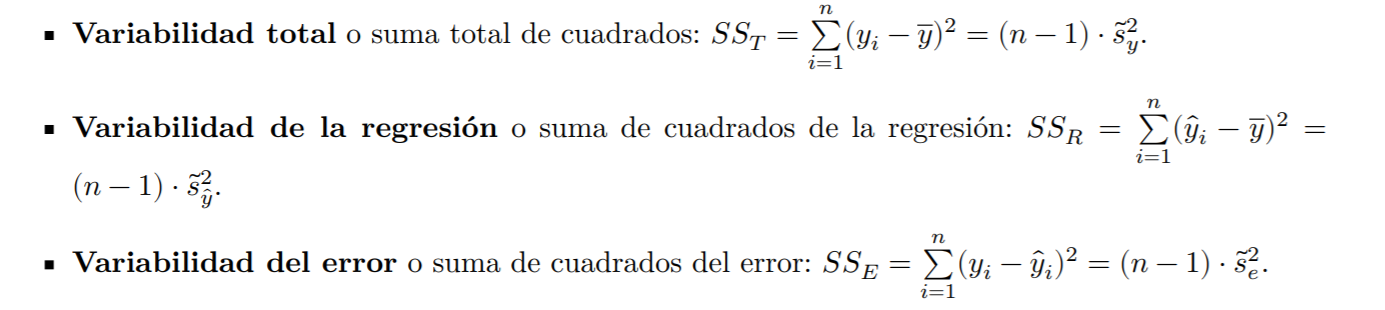
\includegraphics[width=400px]{formulas_regre}

\begin{Shaded}
\begin{Highlighting}[]
\NormalTok{SST=}\KeywordTok{sum}\NormalTok{((y}\OperatorTok{{-}}\KeywordTok{mean}\NormalTok{(y))}\OperatorTok{\^{}}\DecValTok{2}\NormalTok{)}
\NormalTok{SST}
\end{Highlighting}
\end{Shaded}

\begin{verbatim}
## [1] 131.5
\end{verbatim}

\begin{Shaded}
\begin{Highlighting}[]
\KeywordTok{mean}\NormalTok{(y\_est)}
\end{Highlighting}
\end{Shaded}

\begin{verbatim}
## [1] -0.5
\end{verbatim}

\begin{Shaded}
\begin{Highlighting}[]
\KeywordTok{mean}\NormalTok{(y)}\CommentTok{\#media estimados regresión igual a media variable y}
\end{Highlighting}
\end{Shaded}

\begin{verbatim}
## [1] -0.5
\end{verbatim}

\begin{Shaded}
\begin{Highlighting}[]
\NormalTok{SSR=}\KeywordTok{sum}\NormalTok{((y\_est}\OperatorTok{{-}}\KeywordTok{mean}\NormalTok{(y))}\OperatorTok{\^{}}\DecValTok{2}\NormalTok{)}
\NormalTok{SSR}
\end{Highlighting}
\end{Shaded}

\begin{verbatim}
## [1] 126.075
\end{verbatim}

\begin{Shaded}
\begin{Highlighting}[]
\NormalTok{SSE}\CommentTok{\# ya lo había a calculado}
\end{Highlighting}
\end{Shaded}

\begin{verbatim}
## [1] 5.425
\end{verbatim}

\begin{Shaded}
\begin{Highlighting}[]
\NormalTok{SST}\OperatorTok{{-}}\NormalTok{SSR}\CommentTok{\# da lo mismo pues SST=SSR+SSE }
\end{Highlighting}
\end{Shaded}

\begin{verbatim}
## [1] 5.425
\end{verbatim}

\begin{Shaded}
\begin{Highlighting}[]
\NormalTok{R2=SSR}\OperatorTok{/}\NormalTok{SST}
\NormalTok{R2}
\end{Highlighting}
\end{Shaded}

\begin{verbatim}
## [1] 0.9587452
\end{verbatim}

\begin{Shaded}
\begin{Highlighting}[]
\KeywordTok{cor}\NormalTok{(x,y)}
\end{Highlighting}
\end{Shaded}

\begin{verbatim}
## [1] 0.9791554
\end{verbatim}

\begin{Shaded}
\begin{Highlighting}[]
\KeywordTok{cor}\NormalTok{(x,y)}\OperatorTok{\^{}}\DecValTok{2}\CommentTok{\# en el caso regresión simple  R2=cor(xy)\^{}2}
\end{Highlighting}
\end{Shaded}

\begin{verbatim}
## [1] 0.9587452
\end{verbatim}

\hypertarget{problema-12-distribuciuxf3n-de-los-grados-de-un-grafo-de-contactos.}{%
\subsection{Problema 12: Distribución de los grados de un grafo de
contactos.}\label{problema-12-distribuciuxf3n-de-los-grados-de-un-grafo-de-contactos.}}

En el artículo de A. Broder et al.,
\href{http://snap.stanford.edu/class/cs224w-readings/broder00bowtie.pdf}{Graph
structure in the Web. Computer Networks 33, 309 (2000)}.

Se recopiló el número de enlaces a sitios web encontrados en un rastreo
web de 1997 de aproximadamente 200 millones de páginas web,

Con el se construyó una
\href{http://tuvalu.santafe.edu/~aaronc/powerlaws/data/weblinks.hist}{tabla}
con la frecuencia de sitios por número de enlaces. El código siguiente
carga del enlace que han puesto los autores del artículo

\begin{Shaded}
\begin{Highlighting}[]
\NormalTok{data\_links=}\KeywordTok{read.table}\NormalTok{(}\StringTok{"http://tuvalu.santafe.edu/\textasciitilde{}aaronc/powerlaws/data/weblinks.hist"}\NormalTok{,}\DataTypeTok{header=}\OtherTok{TRUE}\NormalTok{)}
\KeywordTok{head}\NormalTok{(data\_links)}
\end{Highlighting}
\end{Shaded}

\begin{verbatim}
##   degree frequency
## 1      0  35159835
## 2      1 106649769
## 3      2  40711748
## 4      3  22648832
## 5      4  12617832
## 6      5   8188854
\end{verbatim}

\begin{Shaded}
\begin{Highlighting}[]
\KeywordTok{str}\NormalTok{(data\_links)}
\end{Highlighting}
\end{Shaded}

\begin{verbatim}
## 'data.frame':    14480 obs. of  2 variables:
##  $ degree   : int  0 1 2 3 4 5 6 7 8 9 ...
##  $ frequency: int  35159835 106649769 40711748 22648832 12617832 8188854 6438634 4690068 4954649 3731928 ...
\end{verbatim}

\begin{Shaded}
\begin{Highlighting}[]
\CommentTok{\# eliminamos la páginas con menos de 8 enlaces  enlaces y las de más de 1000 enlaces}
\NormalTok{data\_links\_central=data\_links[data\_links}\OperatorTok{$}\NormalTok{degree}\OperatorTok{\textgreater{}}\DecValTok{8}\OperatorTok{\&}\NormalTok{data\_links}\OperatorTok{$}\NormalTok{degree}\OperatorTok{\textless{}}\DecValTok{10}\OperatorTok{\^{}}\DecValTok{3}\NormalTok{,]}
\KeywordTok{head}\NormalTok{(data\_links\_central)}
\end{Highlighting}
\end{Shaded}

\begin{verbatim}
##    degree frequency
## 10      9   3731928
## 11     10   3036333
## 12     11   2496648
## 13     12   2119312
## 14     13   1790068
## 15     14   1546579
\end{verbatim}

\begin{Shaded}
\begin{Highlighting}[]
\KeywordTok{tail}\NormalTok{(data\_links\_central)}
\end{Highlighting}
\end{Shaded}

\begin{verbatim}
##      degree frequency
## 995     994       213
## 996     995       193
## 997     996       157
## 998     997       137
## 999     998       178
## 1000    999       153
\end{verbatim}

El siguiente código calcula las regresiones exponencial, potencial y
lineal (en algún orden) de las frecuencias (\texttt{frequency}) contra
los enlaces (\texttt{degree}).

\begin{Shaded}
\begin{Highlighting}[]
\NormalTok{sol1=}\KeywordTok{lm}\NormalTok{(frequency}\OperatorTok{\textasciitilde{}}\StringTok{ }\NormalTok{degree,}\DataTypeTok{data=}\NormalTok{data\_links\_central)}
\KeywordTok{summary}\NormalTok{(sol1)}
\end{Highlighting}
\end{Shaded}

\begin{verbatim}
## 
## Call:
## lm(formula = frequency ~ degree, data = data_links_central)
## 
## Residuals:
##     Min      1Q  Median      3Q     Max 
##  -96861  -69548  -25033   22374 3598744 
## 
## Coefficients:
##              Estimate Std. Error t value            Pr(>|t|)    
## (Intercept) 134974.49   13778.17   9.796 <0.0000000000000002 ***
## degree        -198.98      23.77  -8.369 <0.0000000000000002 ***
## ---
## Signif. codes:  0 '***' 0.001 '**' 0.01 '*' 0.05 '.' 0.1 ' ' 1
## 
## Residual standard error: 214100 on 989 degrees of freedom
## Multiple R-squared:  0.06614,    Adjusted R-squared:  0.06519 
## F-statistic: 70.04 on 1 and 989 DF,  p-value: < 0.00000000000000022
\end{verbatim}

\begin{Shaded}
\begin{Highlighting}[]
\NormalTok{sol2=}\KeywordTok{lm}\NormalTok{(}\KeywordTok{log10}\NormalTok{(frequency)}\OperatorTok{\textasciitilde{}}\StringTok{ }\NormalTok{degree,}\DataTypeTok{data=}\NormalTok{data\_links\_central)}
\KeywordTok{summary}\NormalTok{(sol2)}
\end{Highlighting}
\end{Shaded}

\begin{verbatim}
## 
## Call:
## lm(formula = log10(frequency) ~ degree, data = data_links_central)
## 
## Residuals:
##      Min       1Q   Median       3Q      Max 
## -0.43758 -0.26558 -0.07671  0.16681  2.13097 
## 
## Coefficients:
##                Estimate  Std. Error t value            Pr(>|t|)    
## (Intercept)  4.46504979  0.02381018  187.53 <0.0000000000000002 ***
## degree      -0.00267658  0.00004109  -65.15 <0.0000000000000002 ***
## ---
## Signif. codes:  0 '***' 0.001 '**' 0.01 '*' 0.05 '.' 0.1 ' ' 1
## 
## Residual standard error: 0.37 on 989 degrees of freedom
## Multiple R-squared:  0.811,  Adjusted R-squared:  0.8108 
## F-statistic:  4244 on 1 and 989 DF,  p-value: < 0.00000000000000022
\end{verbatim}

\begin{Shaded}
\begin{Highlighting}[]
\NormalTok{sol3=}\KeywordTok{lm}\NormalTok{(}\KeywordTok{log10}\NormalTok{(frequency)}\OperatorTok{\textasciitilde{}}\StringTok{ }\KeywordTok{log10}\NormalTok{(degree),}\DataTypeTok{data=}\NormalTok{data\_links\_central)}
\KeywordTok{summary}\NormalTok{(sol3)}
\end{Highlighting}
\end{Shaded}

\begin{verbatim}
## 
## Call:
## lm(formula = log10(frequency) ~ log10(degree), data = data_links_central)
## 
## Residuals:
##      Min       1Q   Median       3Q      Max 
## -0.21376 -0.04747 -0.01555  0.01958  0.73976 
## 
## Coefficients:
##                Estimate Std. Error t value            Pr(>|t|)    
## (Intercept)    8.722036   0.020623   422.9 <0.0000000000000002 ***
## log10(degree) -2.170129   0.007894  -274.9 <0.0000000000000002 ***
## ---
## Signif. codes:  0 '***' 0.001 '**' 0.01 '*' 0.05 '.' 0.1 ' ' 1
## 
## Residual standard error: 0.09674 on 989 degrees of freedom
## Multiple R-squared:  0.9871, Adjusted R-squared:  0.9871 
## F-statistic: 7.557e+04 on 1 and 989 DF,  p-value: < 0.00000000000000022
\end{verbatim}

Ahora dibujamos los gráficos adecuados a cada modelo

\begin{Shaded}
\begin{Highlighting}[]
\KeywordTok{plot}\NormalTok{(data\_links\_central,}\DataTypeTok{main=}\StringTok{"Modelo .........."}\NormalTok{)}
\KeywordTok{abline}\NormalTok{(sol1,}\DataTypeTok{col=}\StringTok{"red"}\NormalTok{)}
\end{Highlighting}
\end{Shaded}

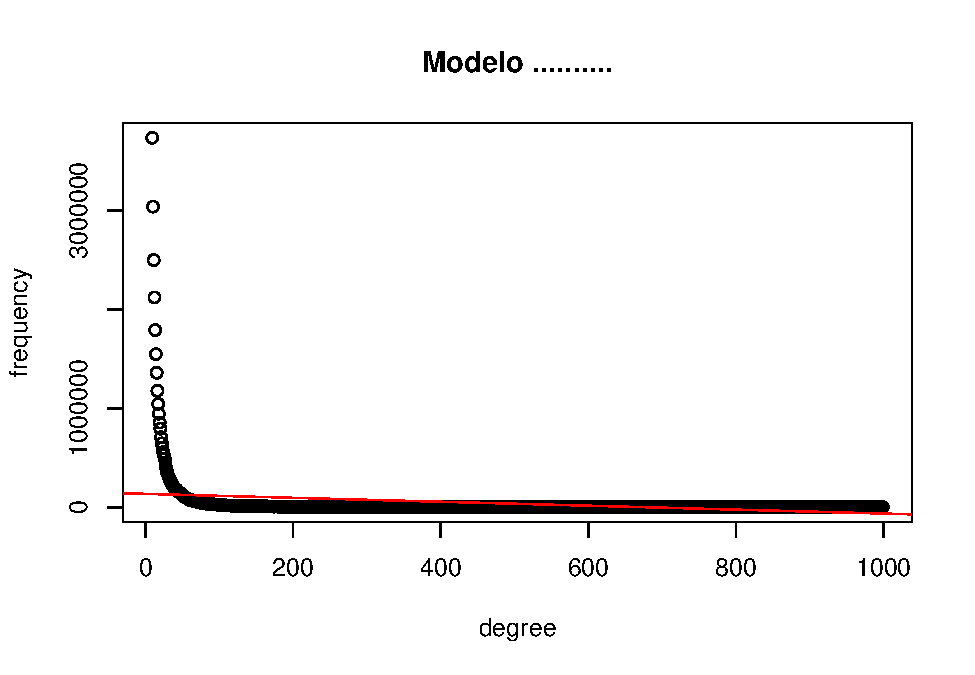
\includegraphics{taller_problemas_resueltos_extra_1_files/figure-latex/unnamed-chunk-53-1.pdf}

\begin{Shaded}
\begin{Highlighting}[]
\KeywordTok{plot}\NormalTok{(data\_links\_central,}\DataTypeTok{main=}\StringTok{"Modelo .........."}\NormalTok{,}\DataTypeTok{log=}\StringTok{"y"}\NormalTok{)}
\KeywordTok{abline}\NormalTok{(sol2,}\DataTypeTok{col=}\StringTok{"red"}\NormalTok{)}
\end{Highlighting}
\end{Shaded}

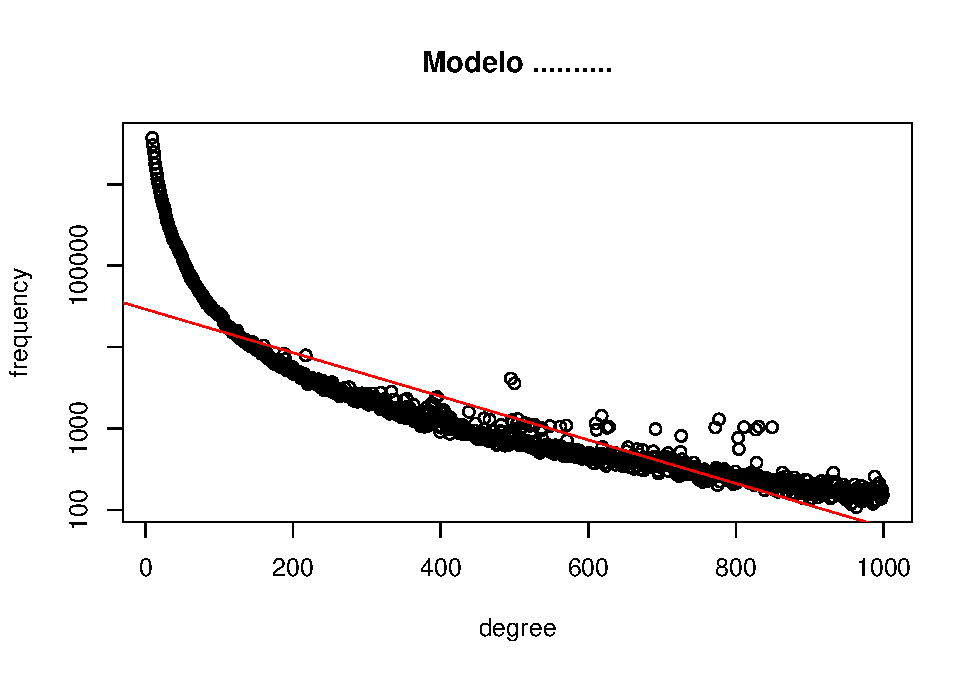
\includegraphics{taller_problemas_resueltos_extra_1_files/figure-latex/unnamed-chunk-53-2.pdf}

\begin{Shaded}
\begin{Highlighting}[]
\KeywordTok{plot}\NormalTok{(data\_links\_central,}\DataTypeTok{main=}\StringTok{"Modelo .........."}\NormalTok{,}\DataTypeTok{log=}\StringTok{"xy"}\NormalTok{)}
\KeywordTok{abline}\NormalTok{(sol3,}\DataTypeTok{col=}\StringTok{"red"}\NormalTok{)}
\end{Highlighting}
\end{Shaded}

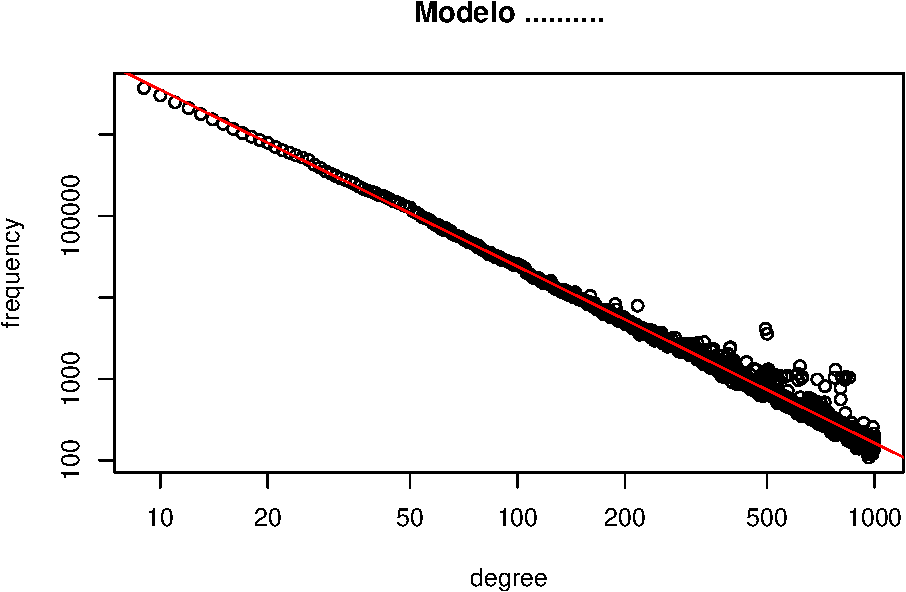
\includegraphics{taller_problemas_resueltos_extra_1_files/figure-latex/unnamed-chunk-53-3.pdf}

Se pide:

\begin{enumerate}
\def\labelenumi{\arabic{enumi}.}
\tightlist
\item
  Explicad el modelo de regresión que calcula cada función \texttt{lm}
\item
  ¿Qué modelo y en función de qué parámetros es el mejor?
\item
  Para el mejor modelo calcular los coeficientes en las unidades
  originales y escribir la ecuación del modelos.
\end{enumerate}

\hypertarget{soluciuxf3n-11}{%
\subsubsection{Solución}\label{soluciuxf3n-11}}

\textbf{Apartado 1}

Los modelos son

\begin{Shaded}
\begin{Highlighting}[]
\NormalTok{sol1=}\KeywordTok{lm}\NormalTok{(frequency}\OperatorTok{\textasciitilde{}}\StringTok{ }\NormalTok{degree,}\DataTypeTok{data=}\NormalTok{data\_links\_central)}
\KeywordTok{summary}\NormalTok{(sol1)}
\end{Highlighting}
\end{Shaded}

\begin{verbatim}
## 
## Call:
## lm(formula = frequency ~ degree, data = data_links_central)
## 
## Residuals:
##     Min      1Q  Median      3Q     Max 
##  -96861  -69548  -25033   22374 3598744 
## 
## Coefficients:
##              Estimate Std. Error t value            Pr(>|t|)    
## (Intercept) 134974.49   13778.17   9.796 <0.0000000000000002 ***
## degree        -198.98      23.77  -8.369 <0.0000000000000002 ***
## ---
## Signif. codes:  0 '***' 0.001 '**' 0.01 '*' 0.05 '.' 0.1 ' ' 1
## 
## Residual standard error: 214100 on 989 degrees of freedom
## Multiple R-squared:  0.06614,    Adjusted R-squared:  0.06519 
## F-statistic: 70.04 on 1 and 989 DF,  p-value: < 0.00000000000000022
\end{verbatim}

\begin{Shaded}
\begin{Highlighting}[]
\NormalTok{sol2=}\KeywordTok{lm}\NormalTok{(}\KeywordTok{log10}\NormalTok{(frequency)}\OperatorTok{\textasciitilde{}}\StringTok{ }\NormalTok{degree,}\DataTypeTok{data=}\NormalTok{data\_links\_central)}
\KeywordTok{summary}\NormalTok{(sol2)}
\end{Highlighting}
\end{Shaded}

\begin{verbatim}
## 
## Call:
## lm(formula = log10(frequency) ~ degree, data = data_links_central)
## 
## Residuals:
##      Min       1Q   Median       3Q      Max 
## -0.43758 -0.26558 -0.07671  0.16681  2.13097 
## 
## Coefficients:
##                Estimate  Std. Error t value            Pr(>|t|)    
## (Intercept)  4.46504979  0.02381018  187.53 <0.0000000000000002 ***
## degree      -0.00267658  0.00004109  -65.15 <0.0000000000000002 ***
## ---
## Signif. codes:  0 '***' 0.001 '**' 0.01 '*' 0.05 '.' 0.1 ' ' 1
## 
## Residual standard error: 0.37 on 989 degrees of freedom
## Multiple R-squared:  0.811,  Adjusted R-squared:  0.8108 
## F-statistic:  4244 on 1 and 989 DF,  p-value: < 0.00000000000000022
\end{verbatim}

\begin{Shaded}
\begin{Highlighting}[]
\NormalTok{sol3=}\KeywordTok{lm}\NormalTok{(}\KeywordTok{log10}\NormalTok{(frequency)}\OperatorTok{\textasciitilde{}}\StringTok{ }\KeywordTok{log10}\NormalTok{(degree),}\DataTypeTok{data=}\NormalTok{data\_links\_central)}
\KeywordTok{summary}\NormalTok{(sol3)}
\end{Highlighting}
\end{Shaded}

\begin{verbatim}
## 
## Call:
## lm(formula = log10(frequency) ~ log10(degree), data = data_links_central)
## 
## Residuals:
##      Min       1Q   Median       3Q      Max 
## -0.21376 -0.04747 -0.01555  0.01958  0.73976 
## 
## Coefficients:
##                Estimate Std. Error t value            Pr(>|t|)    
## (Intercept)    8.722036   0.020623   422.9 <0.0000000000000002 ***
## log10(degree) -2.170129   0.007894  -274.9 <0.0000000000000002 ***
## ---
## Signif. codes:  0 '***' 0.001 '**' 0.01 '*' 0.05 '.' 0.1 ' ' 1
## 
## Residual standard error: 0.09674 on 989 degrees of freedom
## Multiple R-squared:  0.9871, Adjusted R-squared:  0.9871 
## F-statistic: 7.557e+04 on 1 and 989 DF,  p-value: < 0.00000000000000022
\end{verbatim}

Así que

\begin{itemize}
\tightlist
\item
  el primero es \(frequency = b_0+b_1\cdot degree\) que es el modelo
  LINEAL que resuelve la función \texttt{lm}.
\item
  el segundo es \(\log_{10}(frequency) = b_0+b_1\cdot degree\) que
  operando adecuadamente es
\end{itemize}

\(10^{\log_{10}(frequency)}=10^{b_0}\cdot 10^{b_1\cdot degree}\)
operando obtenemos que el modelo final es un modelo EXPONENCIAL
\(frequency=10^{b_0}\cdot \left(10^{b_1}\right)^{degree}\). * el tercer
modelo es \(\log_{10}(frequency) = b_0+b_1\cdot \log_{10}(degree)\) que
despejando es
\(10^{\log_{10}(frequency)}=10^{b_0}\cdot \left(10^{\left(\log_{10}(degree)\right)}\right)^{b_1}\)
operando obtenemos que el modelo final es un modelo POTENCIAL
\(frequency=10^{b_0}\cdot degree^{b_1}.\)

Los dibujos con el título adecuado son

\begin{Shaded}
\begin{Highlighting}[]
\KeywordTok{plot}\NormalTok{(data\_links\_central,}\DataTypeTok{main=}\StringTok{"Modelo lineal"}\NormalTok{)}
\KeywordTok{abline}\NormalTok{(sol1,}\DataTypeTok{col=}\StringTok{"red"}\NormalTok{)}
\end{Highlighting}
\end{Shaded}

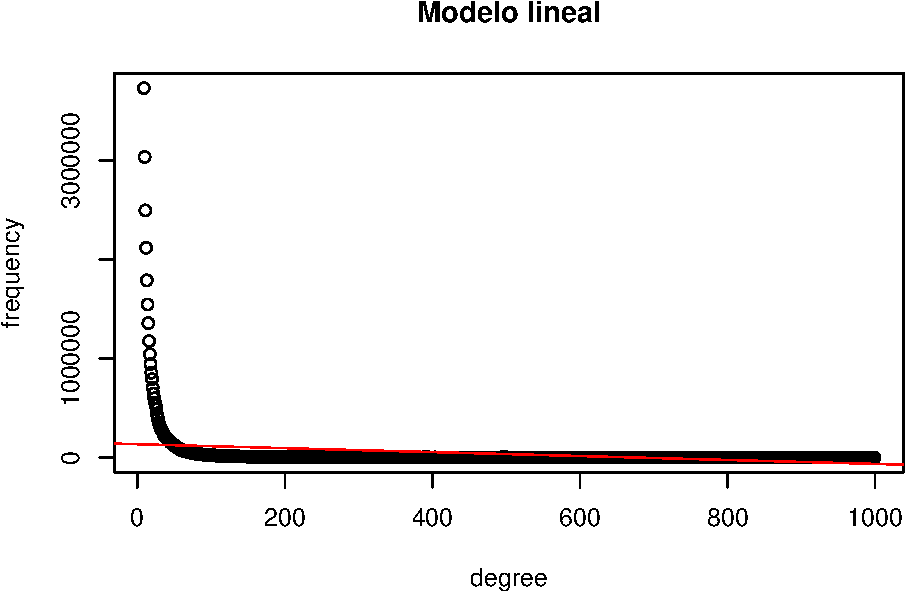
\includegraphics{taller_problemas_resueltos_extra_1_files/figure-latex/unnamed-chunk-55-1.pdf}

\begin{Shaded}
\begin{Highlighting}[]
\KeywordTok{plot}\NormalTok{(data\_links\_central,}\DataTypeTok{main=}\StringTok{"Modelo exponencial"}\NormalTok{,}\DataTypeTok{log=}\StringTok{"y"}\NormalTok{)}
\KeywordTok{abline}\NormalTok{(sol2,}\DataTypeTok{col=}\StringTok{"red"}\NormalTok{)}
\end{Highlighting}
\end{Shaded}

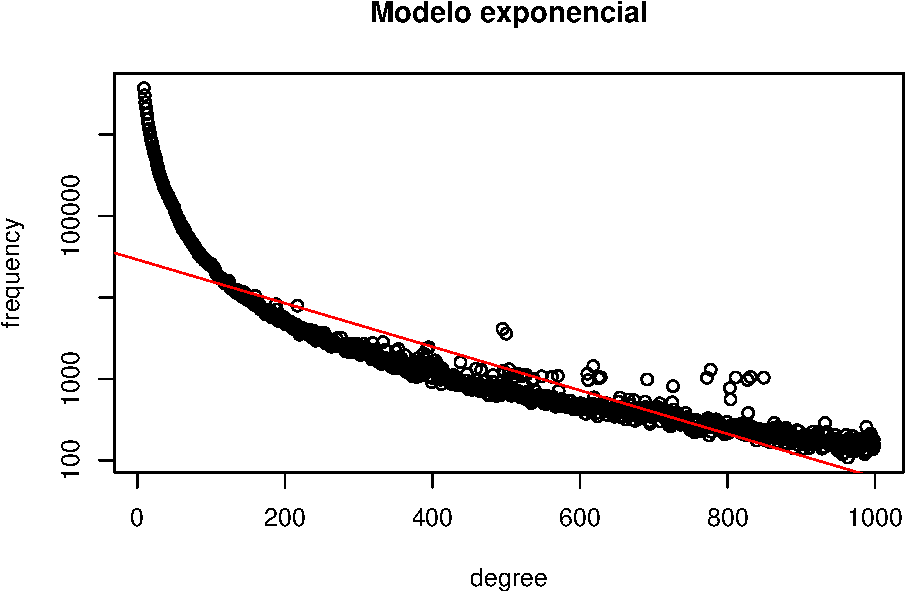
\includegraphics{taller_problemas_resueltos_extra_1_files/figure-latex/unnamed-chunk-55-2.pdf}

\begin{Shaded}
\begin{Highlighting}[]
\KeywordTok{plot}\NormalTok{(data\_links\_central,}\DataTypeTok{main=}\StringTok{"Modelo potencial"}\NormalTok{,}\DataTypeTok{log=}\StringTok{"xy"}\NormalTok{)}
\KeywordTok{abline}\NormalTok{(sol3,}\DataTypeTok{col=}\StringTok{"red"}\NormalTok{)}
\end{Highlighting}
\end{Shaded}

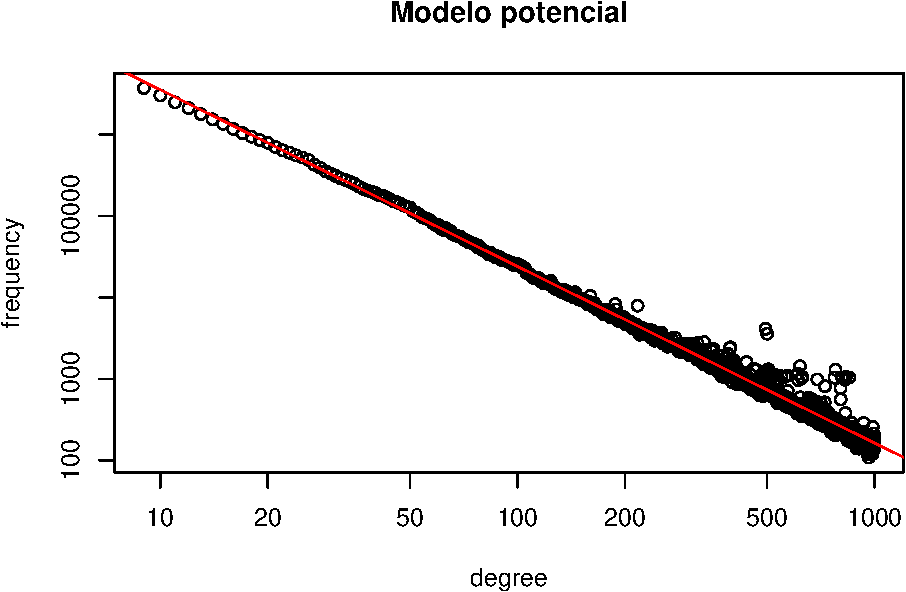
\includegraphics{taller_problemas_resueltos_extra_1_files/figure-latex/unnamed-chunk-55-3.pdf}

Con lo que hemos visto el modelo con mejor \(R^2\) es el mejor

\begin{Shaded}
\begin{Highlighting}[]
\KeywordTok{summary}\NormalTok{(sol1)}\OperatorTok{$}\NormalTok{r.squared}
\end{Highlighting}
\end{Shaded}

\begin{verbatim}
## [1] 0.06613879
\end{verbatim}

\begin{Shaded}
\begin{Highlighting}[]
\KeywordTok{summary}\NormalTok{(sol2)}\OperatorTok{$}\NormalTok{r.squared}
\end{Highlighting}
\end{Shaded}

\begin{verbatim}
## [1] 0.8110118
\end{verbatim}

\begin{Shaded}
\begin{Highlighting}[]
\KeywordTok{summary}\NormalTok{(sol3)}\OperatorTok{$}\NormalTok{r.squared}
\end{Highlighting}
\end{Shaded}

\begin{verbatim}
## [1] 0.9870815
\end{verbatim}

Así que el mejor modelo es el tercero el potencial pues su \(R^2\) es
muy alto

\textbf{Apartado 3}

Calcularemos la ecuación del modelo para las unidades originales sin
transformaciones logarítmicas.

Recordemos el resultado de la \texttt{sol3}

\begin{Shaded}
\begin{Highlighting}[]
\KeywordTok{summary}\NormalTok{(sol3)}
\end{Highlighting}
\end{Shaded}

\begin{verbatim}
## 
## Call:
## lm(formula = log10(frequency) ~ log10(degree), data = data_links_central)
## 
## Residuals:
##      Min       1Q   Median       3Q      Max 
## -0.21376 -0.04747 -0.01555  0.01958  0.73976 
## 
## Coefficients:
##                Estimate Std. Error t value            Pr(>|t|)    
## (Intercept)    8.722036   0.020623   422.9 <0.0000000000000002 ***
## log10(degree) -2.170129   0.007894  -274.9 <0.0000000000000002 ***
## ---
## Signif. codes:  0 '***' 0.001 '**' 0.01 '*' 0.05 '.' 0.1 ' ' 1
## 
## Residual standard error: 0.09674 on 989 degrees of freedom
## Multiple R-squared:  0.9871, Adjusted R-squared:  0.9871 
## F-statistic: 7.557e+04 on 1 and 989 DF,  p-value: < 0.00000000000000022
\end{verbatim}

Los estimadores son \(b_0=8.722036\) y \(b_1=-2.170129\) el modelo es
\(frequency=10^{b_0}\cdot degree^{b_1}\). Sustituyendo los valores el
modelo obtenemos \(frequency=10^{8.722036}\cdot degree^{-2.170129}\),
finalmente operando

\[frequency=527273566.93254\cdot degree^{-2.170129}.\]

No se pedía en el ejercicio pero hacemos el dibujo de los datos y la
ecuación en las unidades originales

\begin{Shaded}
\begin{Highlighting}[]
\NormalTok{frequency=data\_links\_central}\OperatorTok{$}\NormalTok{frequency}
\NormalTok{degree=data\_links\_central}\OperatorTok{$}\NormalTok{degree}
\NormalTok{potencial=}\ControlFlowTok{function}\NormalTok{(x) }\DecValTok{10}\OperatorTok{\^{}}\NormalTok{(}\FloatTok{8.722036}\NormalTok{)}\OperatorTok{*}\NormalTok{x}\OperatorTok{\^{}}\NormalTok{(}\OperatorTok{{-}}\FloatTok{2.170129}\NormalTok{)}
\KeywordTok{plot}\NormalTok{(degree,frequency,}\DataTypeTok{main=}\StringTok{"Modelo potencial"}\NormalTok{,}\DataTypeTok{xlab=}\StringTok{"degree"}\NormalTok{,}\DataTypeTok{ylab=}\StringTok{"frequency"}\NormalTok{)}
\KeywordTok{curve}\NormalTok{(potencial,}\DataTypeTok{xlim=}\KeywordTok{c}\NormalTok{(}\DecValTok{0}\NormalTok{,}\DecValTok{1000}\NormalTok{),}\DataTypeTok{ylim=}\KeywordTok{c}\NormalTok{(}\DecValTok{0}\NormalTok{,}\DecValTok{3731928}\NormalTok{),}\DataTypeTok{col=}\StringTok{"red"}\NormalTok{,}\DataTypeTok{add=}\OtherTok{TRUE}\NormalTok{)}
\end{Highlighting}
\end{Shaded}

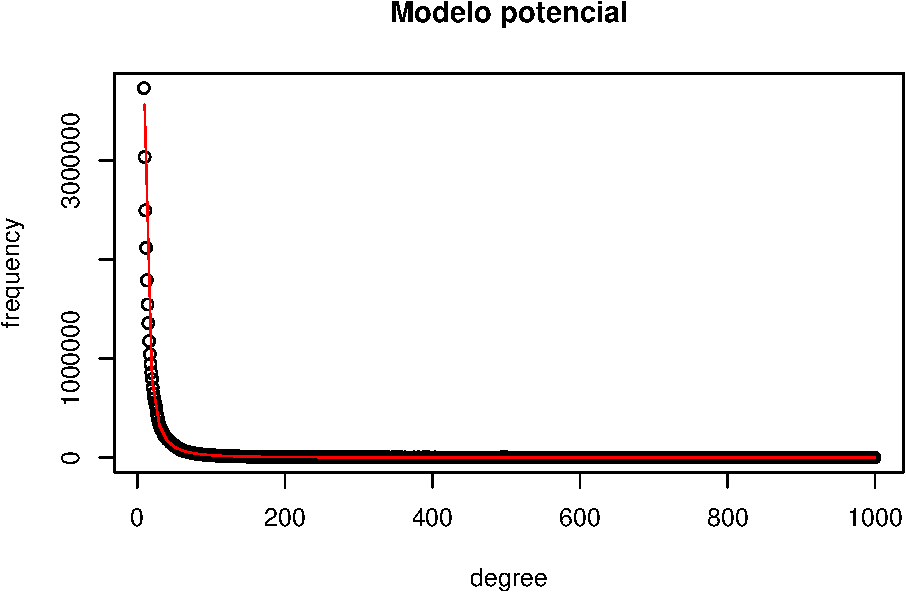
\includegraphics{taller_problemas_resueltos_extra_1_files/figure-latex/unnamed-chunk-58-1.pdf}

\end{document}
